\chapter{DemVR: Public Engaged Hackathon}
\label{DemVR}

\section{Introduction}
\label{sec:DemVRIntroduction}



The study covered in this chapter is currently being peer-reviewed in the TOCHI journal. The paper is co-authored by Dr. Sarah Foley, Dr. Daniel Lambton-Howard, Dr. Kyle Montague, Dr. Laura Booi, Sandra Hastings, Prof. David Kirk, and Dr. Kellie Morrissey. I was responsible for concept, study design, data collection, data analysis and writing of the paper. Co-authors supported the facilitation of the hackathon, and Dr. Kellie Morrissey, Dr. Sarah Foley and Dr. David Kirk provided feedback on the paper's writing and contribution.

\section{Event context}
\label{sec:DemVRContextEvent}

\begin{figure}
\centering
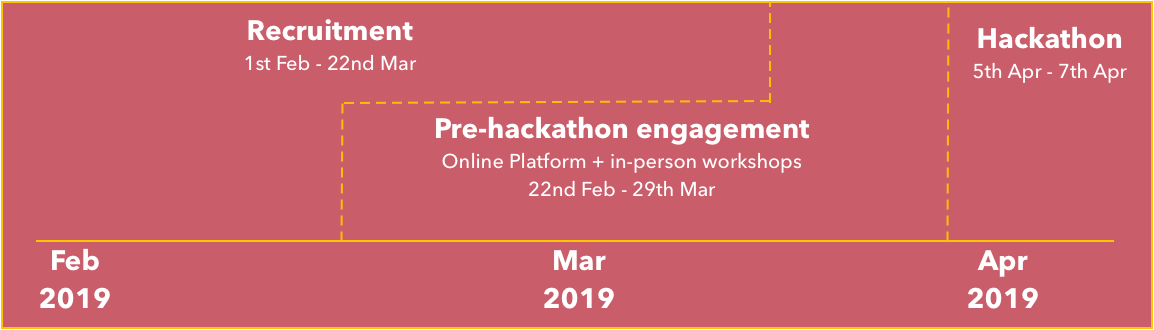
\includegraphics[width=.8\linewidth]{Images/Timeline.jpg}
\caption{Timeline of the event}
\label{fig:DemVRTimeline}
\end{figure}

In 2019, I set out to organise a hackathon called DemVR, both to generate a set of bespoke VR environments for those living with dementia, as well as to consider how developers/designers (with expertise in media or VR) and people living with dementia may collaborate. Inspired by prior work involving lived experiences in hackathons \citep{birbeck_self_2017}, the hackathon was split into two engagement phases see Fig.\ref{fig:DemVRTimeline}. The first was a six-week pre-hackathon phase: this consisted of the deployment of an online platform (called Ideaboard) to support designers/developers in pitching their potential hackathon ideas and receiving feedback from people living with dementia and care partners. The second phase was the two-day hackathon event itself, where participants formed teams to compete for £1,000 \& £500 prizes by creating prototypes of VR experiences for people living with dementia and their care partners. To accommodate funding for venue hire, branding, food and travel, I partnered up with several organisations in Newcastle who assisted in the funding and providing expert knowledge on dementia, VR, and running tech-focused events. For instance, continuing my relationship with Silvelrine Memories provided the hackathon with dementia expertise, while connecting with Sunderland Software City provided funding for venue hire. In this section below, I will describe the following: pre-hackathon phase, hackathon, recruitment, final team ideas, and finally a reflection on running the event.

\subsection{Pre-hackathon engagement}
\label{sec:EventPrehackathon}
I planned and arranged a six-week consultation period, to be carried out via 1) an online participatory platform, and 2) in-person workshops with people living with dementia, and their care partners. Both components of the pre-hackathon phase was in hope that this would allow people who might be unavailable for the hackathon to still take part in design ideation and help to shape emerging ideas which would then be taken further in the in-person hackathon. Below, I describe first what Ideaboard is, and second, the in-person workshops. Finally, the day before our hackathon event, I held a team formation event, where hackathon participants could freely attend to explore published ideas and form teams if they had not done already. During the evening formation event, I printed the eleven ideas published on Ideaboard and placed them on individual tables with sticky notes for participants to add any further comments or express interest in the idea. Since submitting ideas on Ideaboard was optional, five teams came prepared with ideas. As a result, only four of the eleven Ideaboard posts were taken into the hackathon. 

\subsubsection{Ideaboard}
\label{sec:Ideaboard}
The participatory platform, Ideaboard\footnote{www.Ideaboard.co.uk}, was conceptually developed in-house at Open Lab from prior participatory platforms in working in Digital Civics and social care - for instance, one inspiration was App Movement \citep{garbett_app_2016}, a platform that enables users to \textit{"collaborate, design, and deploy community commissioned mobile applications"}. Similarly, Ideaboard offers creative tools and workspaces to support the creation of ideas and collaboration. Interested in deploying Open Lab's bespoke tools in an attempt to engaging with designers and people living with dementia, I deployed Ideaboard to be the central platform that was used for the six-week pre-hackathon engagement phase. 

Here, I describe the process users undertake to add ideas to the platform. On Ideaboard, participants were invited to share preliminary ideas that they could develop during the in-person hackathon. Users would upload an idea providing a title, tagline, description and an optional banner image. Once uploaded, users could freely navigate the Ideaboard 'Explore' page to read and comment on other submitted ideas (see Fig.\ref{fig:exploreIdeaboard}). Once designers/developers had submitted their ideas, I then invited people with dementia and their care partners (recruitment described in section \ref{sec:EventRecruitment}) to share insights and critique the submitted ideas before the hackathon. 

\begin{figure}
\centering
\begin{subfigure}{.5\textwidth}
  \centering
  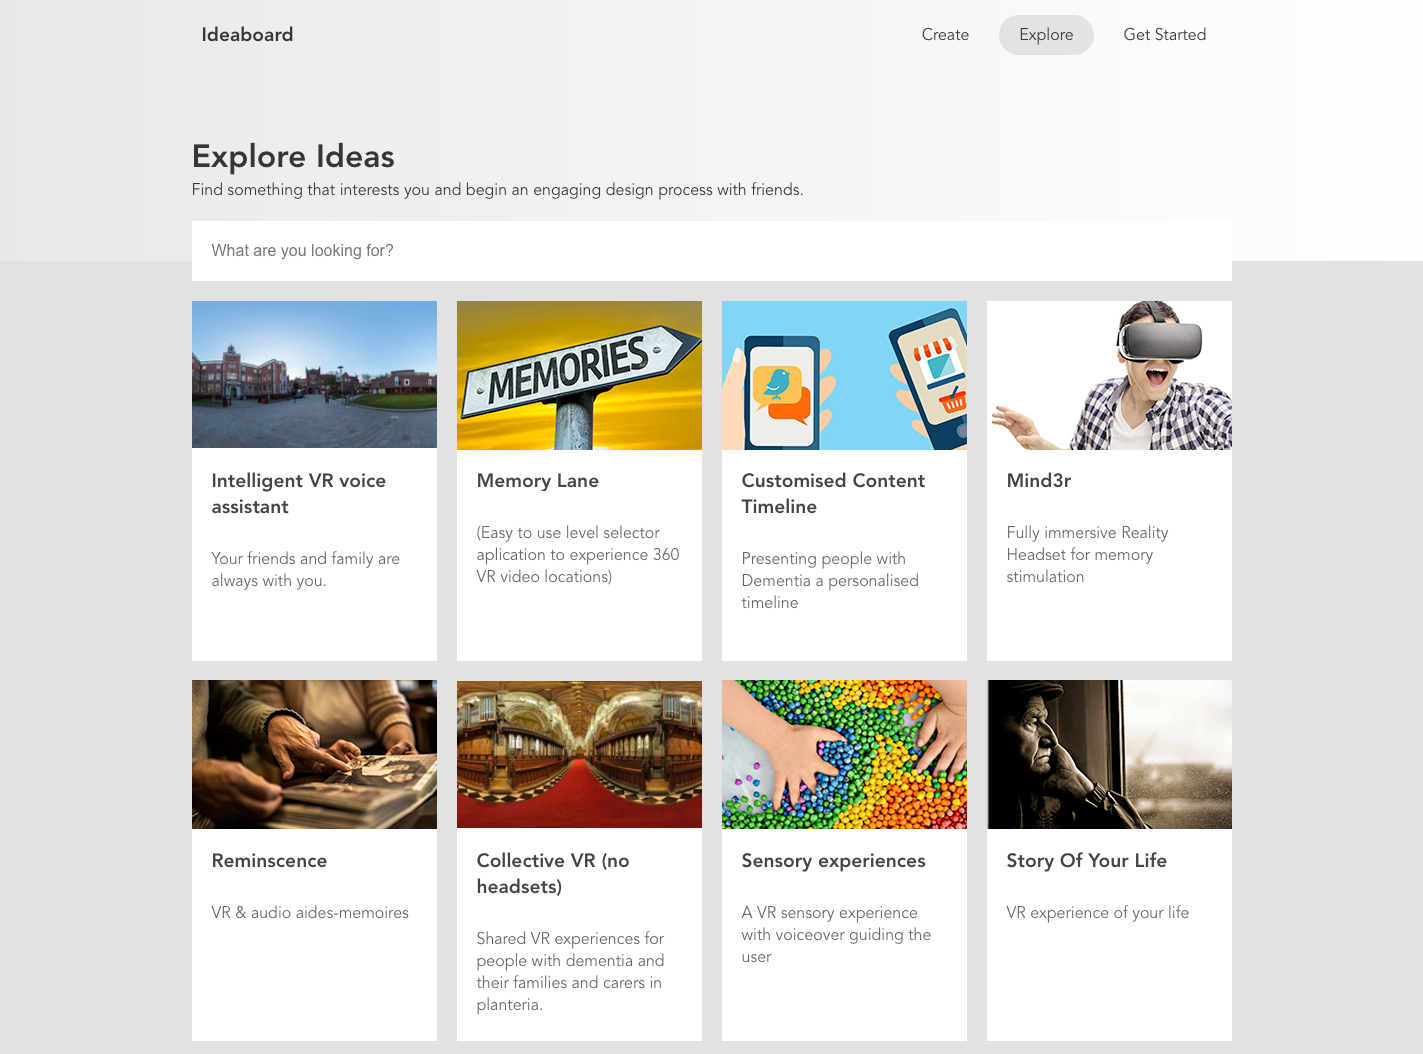
\includegraphics[width=.8\linewidth]{Images/Ideaboard Ideas.png}
  \caption{Explore Ideaboard ideas}
  \label{fig:exploreIdeaboard}
\end{subfigure}%
\begin{subfigure}{.5\textwidth}
  \centering
  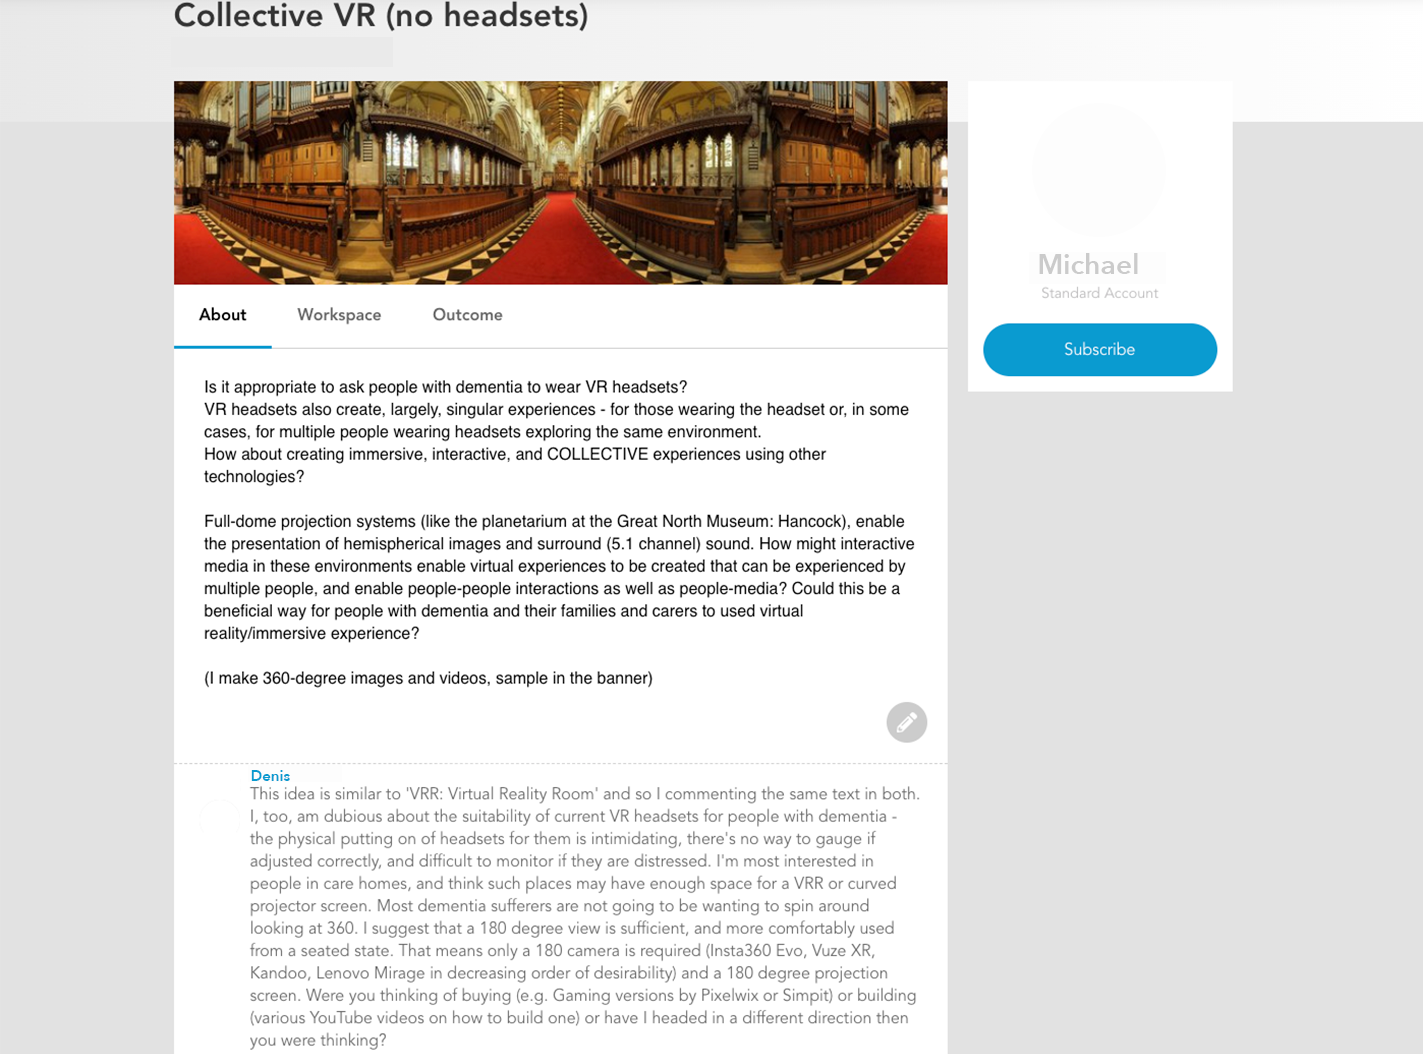
\includegraphics[width=.8\linewidth]{Images/Example of idea.png}
  \caption{Example of 'idea' features}
  \label{fig:IdeaboardIdea}
\end{subfigure}
\caption{Ideaboard features}
\label{fig:IdeaboardFeatures}
\end{figure}

\subsubsection{In-person workshops}
\label{sec:in-personWorkshops}
Concerned by a number of participants in my prior work rarely used social media or online platforms, I set up two in-person workshop sessions inviting members of Silverline Memories with the aim to ensure their feedback and thoughts were provided in the event. During the workshops, participants would participate in a set of design activities to illustrate their desired VR shared experiences or build upon the existing eleven ideas posted on Ideaboard. Based on comments and ideas produced in these workshops by care partners and people living with dementia, I would then add any additional ideas to Ideaboard or add any comments made about existing ideas to the relevant Ideaboard idea. By returning the ideas back to Ideaboard, this would ensure the event would have a consistent 'hub' for thoughts and ideas of creating VR experiences for people with dementia. Further, the addition of ideas from Silverline Memories would allow designers/developers to have additional time to reflect on comments from people living with dementia and their care partners prior to the two-day event. However, as stated throughout this chapter, our attempts to involve people living with dementia and their care partners was significantly limited to only one care partner engaging on the online platform. 

\subsection{Hackathon}
The hackathon too place across one weekend (April 5\textsuperscript{th} - 7\textsuperscript{th} 2019), at a local museum in Newcastle. In terms of equipment, teams had access to eight Oculus Go's, four Oculus Rifts, one HTC Vive, and two VR-ready PC rigs. Teams were encouraged to bring laptops and VR kit if they wished, and to notify the facilitators before the event if they need any particular additional technologies to be provided. The first morning of the event consisted of presentations on dementia, participatory research, and virtual reality by invited speakers. Due to the lack of engagement at our in-person workshops, we organised an online Q\&A with Howard, a dementia advocate who shared his experiences living with dementia. As Howard was unavailable to travel to Newcastle for the weekend, he joined by Zoom on the Saturday afternoon for a duration of 15 minutes (see fig.\ref{fig:Howard}. 


\begin{figure}
\centering
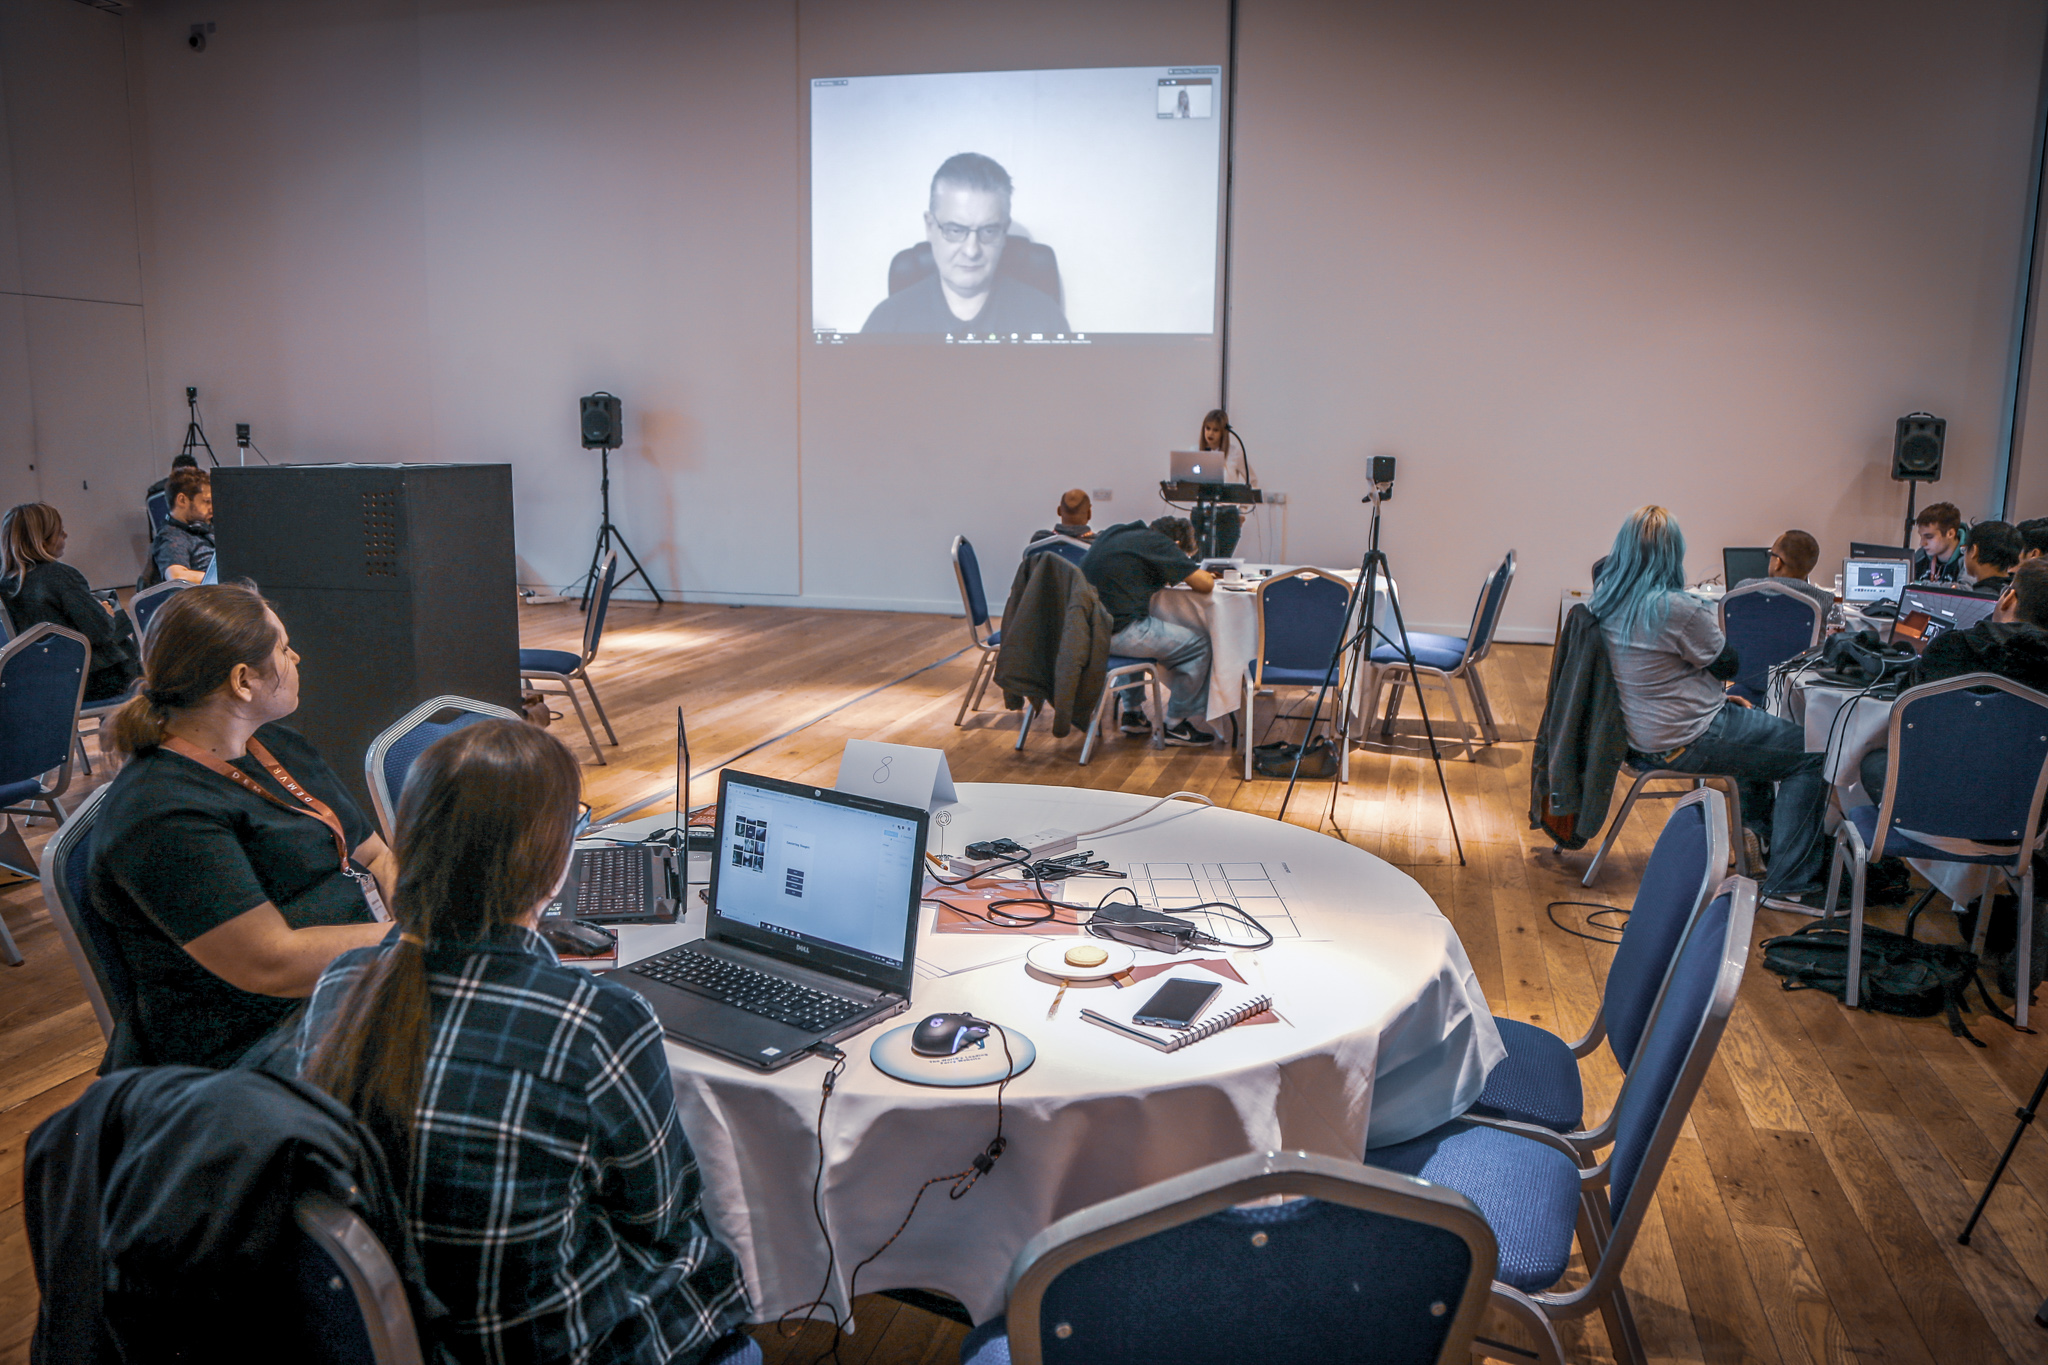
\includegraphics[width=.8\linewidth]{Images/Howard.jpg}
\caption{Howard's Zoom Q\&A}
\label{fig:Howard}
\end{figure}

Throughout the two days, teams could ask for additional help or critique from the available facilitators (described in \ref{sec:EventRecruitment}, via in-person or reaching out to the facilitators in the individually set up WhatsApp team groups. Within these groups, teams were asked to document and audio record answers to a series of questions we asked throughout the two days. For example, questions consisted of: \textit{"sum up some of the issues \& themes you've been discussing this morning"}, \textit{"describe your reaction to Howard's Q\&A"}, and \textit{"what is one thing you've learned from this weekend that you didn't know at the beginning of day one?"}. Further, these WhatsApp groups, teams were also invited to detail their project's progression through submitting comments, audio recordings and videos through their dedicated group chat, which formed the basis of data collected during the event. To encourage teams to think about designing VR experiences for people with dementia, I provided them with \textit{inspiration packs} seen in fig.\ref{fig:InspirationPacks}: these consisted of materials that summarized key insights from previously published work on VR and dementia \citep{hodge_exploring_2018,hodge_exploring_2019}. 

\begin{figure}
\centering
\begin{subfigure}{.5\textwidth}
  \centering
  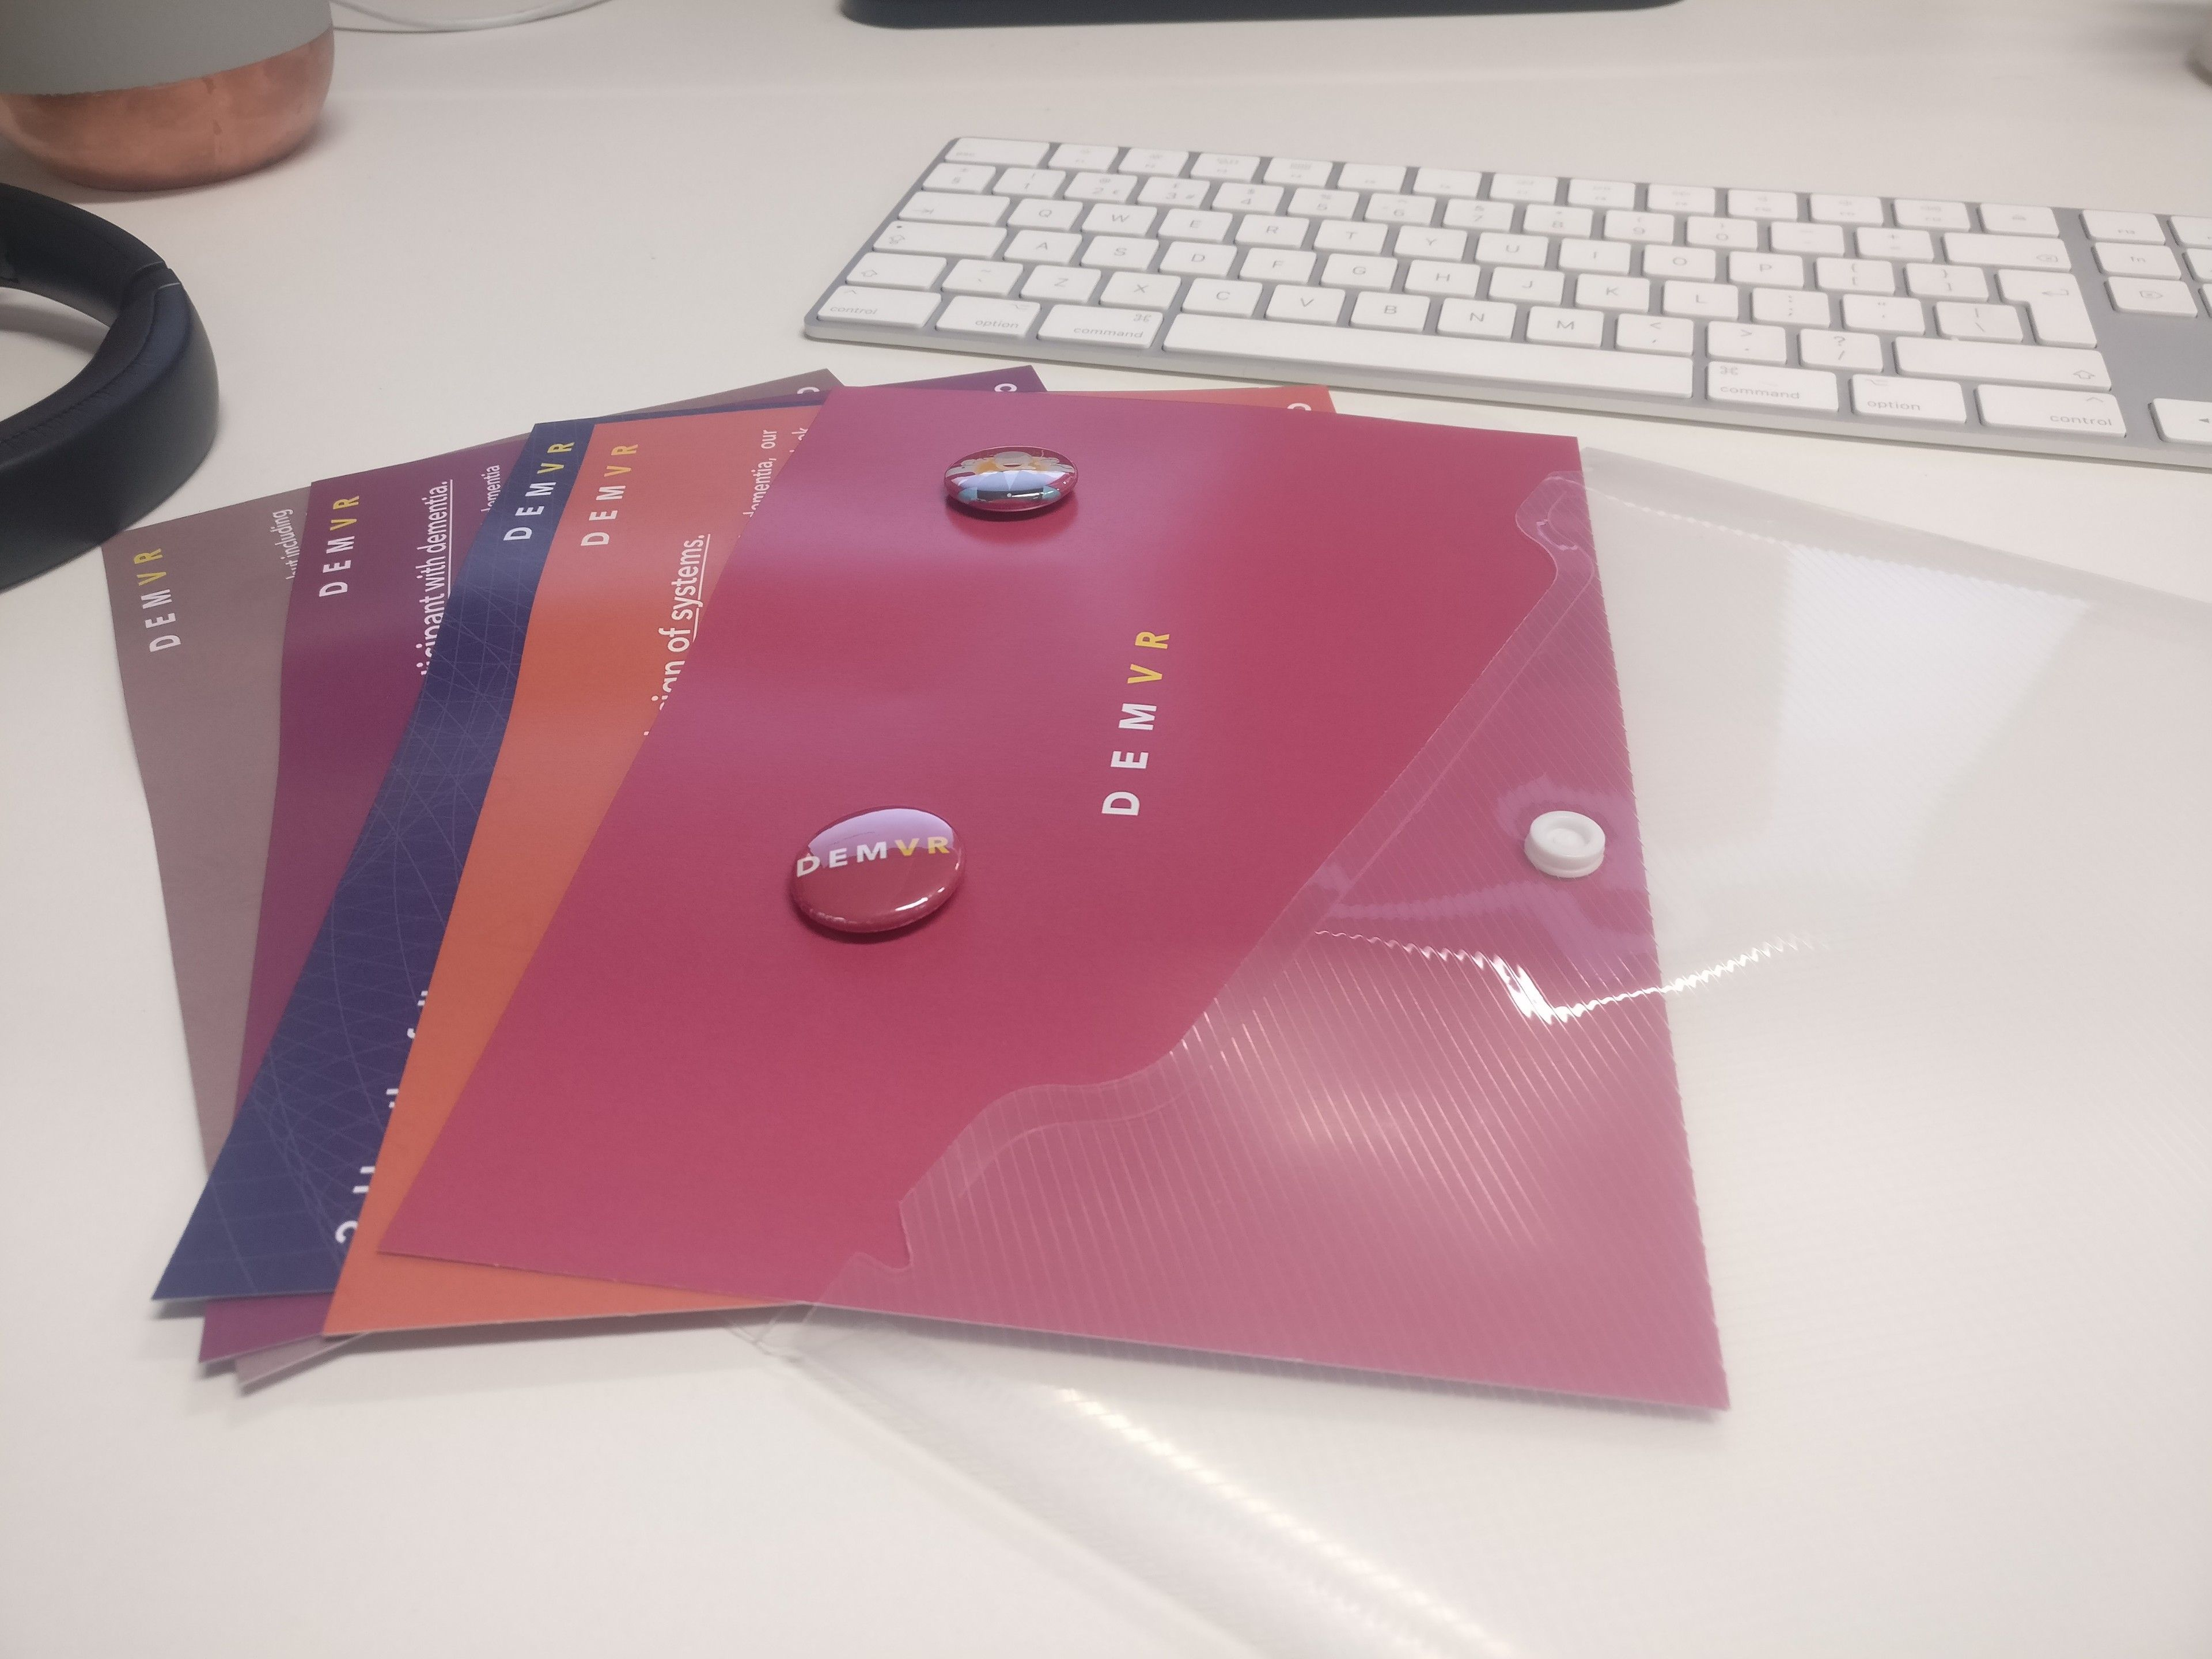
\includegraphics[width=.8\linewidth]{Images/DemVRInspiration.jpeg}
  \label{fig:InspirationPackImage}
\end{subfigure}%
\begin{subfigure}{.5\textwidth}
  \centering
  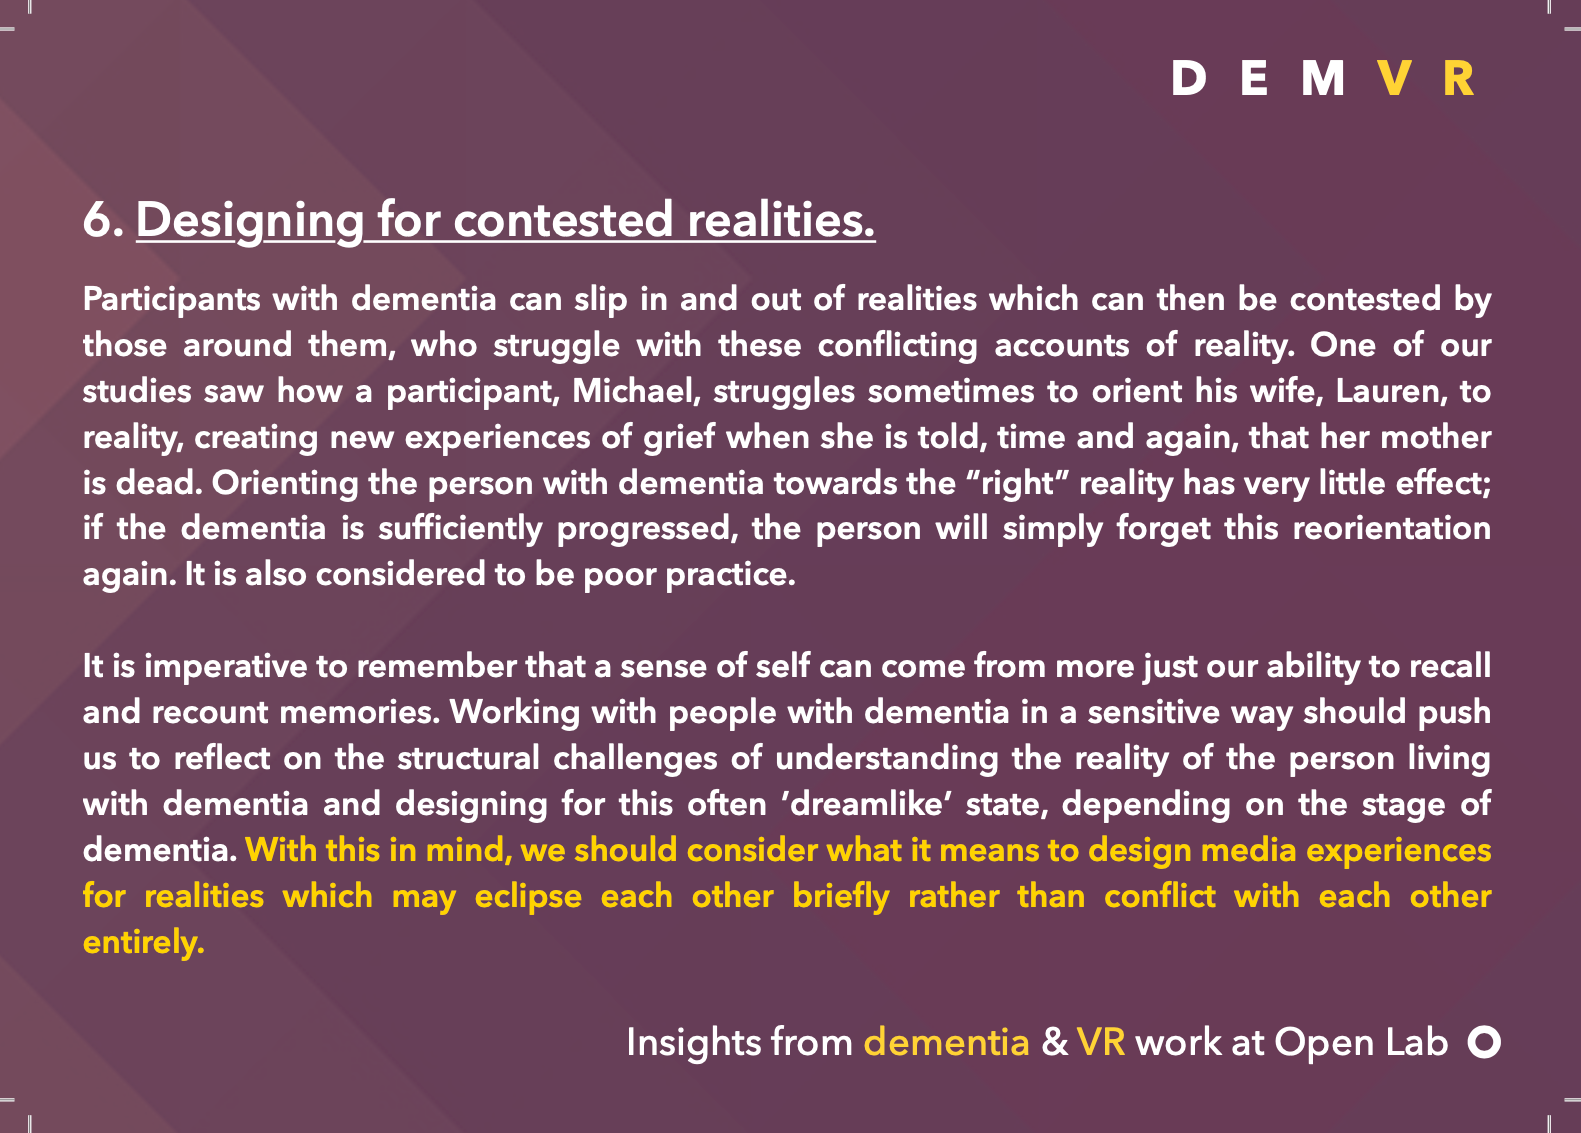
\includegraphics[width=.8\linewidth]{Images/InspirationCard.png}
  \label{fig:InspirationCard}
\end{subfigure}
\caption{Inspiration packs}
\label{fig:InspirationPacks}
\end{figure}

In addition to the physical inspiration packs, I set up an online shared document that continued to grow as a resources through the duration of the event. In the end, this documentation consisted of academic papers; speaker slides; dementia guides such as DEEP language and NHS guides; a set of design method processes such as scenarios, bodystorming, and 5 Whys; and tips and tricks for what to include in the final presentation. For the rest of the weekend, the teams worked on their ideas with periods built in for breaks ans socialisation see fig.\ref{fig:schedule}. The event culminated in a final ten-minute presentation and five-minute demo at the end of day two in which the teams demonstrated their work to the judges. Participants' finalised concepts were rated on the following: 1) novelty of design, 2) clarity of team's vision, 3) sensitivity to the challenge, 4) potential for real-world impact, and 5) strength of VR/AR.

\begin{figure}
\centering
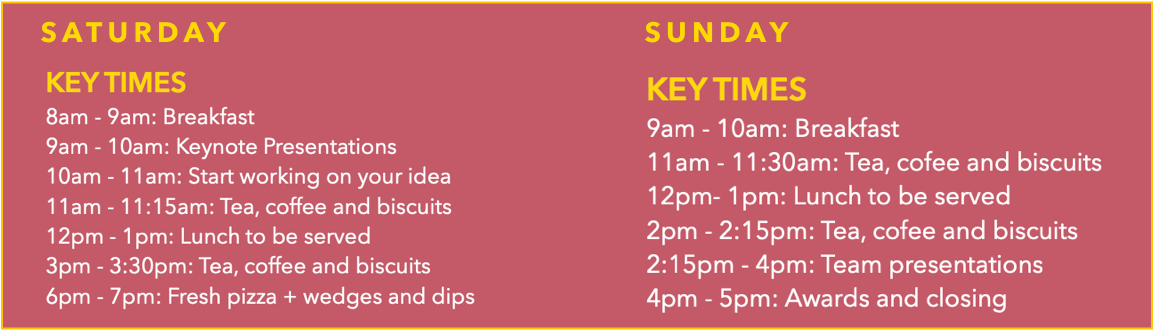
\includegraphics[width=.8\linewidth]{Images/DemVRHackathonSchedule.jpg}
\caption{DemVR schedule}
\label{fig:schedule}
\end{figure}

\subsection{Recruitment}
\label{sec:EventRecruitment}
My initial recruitment process targeted designers and developers through university networks, VR/AR labs across the UK, as well as publishing blog pieces on popular VR websites to invite creators to take part in the two-day event. Upon registering for the event on our website\footnote{www.demvr.uk}, participants were sent an email inviting them to sign up for Ideaboard and submit their idea, I attempted to recruit people living with dementia and their care partners in multiple ways. The first, was through Silverline Memories who I talk in detail about in chapter \ref{NegotatingReseacherParticipantRelationships}. Secondly, given Twitter is a popular social media platform for dementia network and advocates \citep{talbot_how_2020}, I ran a Twitter account posting tweets to encourage people living with dementia and their care partners to sign-up. In these instances, while I invited people with dementia and care partners to the hackathon, the priority was signing them up to the online platform or take part in the in-person workshops as the pre-engagement phase supported longer-term engagement. However, as I mentioned in this chapter, our recruitment process to involve people living with dementia and care partners failed with only one care partner signing up to our platform.

For those without experience of dementia, twelve participants (2 women, 10 men) actively signed up to the online platform. During set up, to get the conversation rolling, I added three initial example ideas focused on shared family VR environments, personalising the VR headset, and a VR experience that blends the real world and virtual into one. Out of the twelve participants, eight submitted ideas. Of the twelve participants, nine attended the hackathon (see table \ref{table:DemVRDemographic}), with two of them submitting an idea but not attending the hackathon. One participant, a care partner named Denis, was unable to attend the hackathon but actively joined discussions on six of the submitted ideas. Additionally, while we set-up two in-person workshops described in \ref{sec:EventPrehackathon}, the workshops received no sign-ups resulting in no additional feedback for teams from people living with dementia or their care partners. In the following sections, I dive into this further considering why this may have been the case. 

For the hackathon, I had 40 participants (18 women, 22 men) attend. In our pre-hackathon team formation stage, I had an additional team of four that dropped out due to intellectual property concerns. This resulted in nine teams. Individual demographics of participants within their associated teams are summarised in table \ref{table:DemVRDemographic}. Although no participants had the experience of being a care partner or living with dementia, participants identified their experience with dementia during the sign-up process from the following: 

\begin{itemize}
\item{\textbf{Experienced}: worked in the area of dementia in a research/industry/care setting/charity.}
\item{\textbf{Knowledgeable}: Has had a family member or friend living with dementia but not necessarily cared for them.}
\item{\textbf{Limited}: Have read people's experiences or recent research in the area of dementia.}
\item{\textbf{None}: Know very little about the topic}
\end{itemize}

% custom commands
\newcolumntype{L}[1]{>{\raggedright\let\newline\\\arraybackslash\hspace{0pt}}p{#1}}
\newcolumntype{C}[1]{>{\centering\let\newline\\\arraybackslash\hspace{0pt}}p{#1}}
\newcolumntype{R}[1]{>{\raggedleft\let\newline\\\arraybackslash\hspace{0pt}}p{#1}}

% this line fixes the vertical padding of text inside the cells
\renewcommand{\arraystretch}{1.4}

\begin{table*}[!ht]
\begin{tabularx}{\textwidth}{@{} YYYYYY @{}}
\hline
\textbf{Team} & \textbf{No. members} & \textbf{Age range} & \textbf{Background} & \textbf{Experience with dementia} & \textbf{No. Ideaboard\footnote{members who joined Ideaboard}} \\ \hline 
Garden Life & 7 & 16-25 & Comp-sci undergrads (7) & Limited (1) / None (6) & 3 \\ \hline
Chatter Bench & 2 & 26-45 & History researcher (1) / HCI research developer   (1) & Experienced (1) / Limited (1) & 0 \\ \hline
Augmented World & 6 & 16-25 & Comp-sci undergrads (6) & Limited (2) / None (4) & 1 \\ \hline
VRHallucinate & 6 & 16-35 & Psychology researcher (2) / Developer (3) /   Designers (1) & Limited (1) / None (5) & 0 \\ \hline
LookingVRBack & 4 & 25-45 & Marketing (1) / Biomedical researcher (1) /   Comp-sci undergrad (2) & Experienced (1) / None (3) & 2 \\ \hline
Mindful Forest & 2 & 16-25 & Comp-sci undergrad (2) & Passing (2) & 0 \\ \hline
Sensory Tide & 6 & 26-45 & HCI researcher (3) / Developer (1) / Filmmaker   (2) & Experienced (2) / Passing (1) / None (2) & 3 \\ \hline
World Share & 3 & 16-25 & Filmmaker (3) & Passing (1) / None (2) & 0 \\ \hline
VRmotion & 4 & 16-25 & HCI researcher (1) / Developer (1) / Designer   (2) & Experienced (1) / Limited (1) / None (2) & 0 \\ \hline
\end{tabularx}
\caption{Here is a caption.}
\label{table:DemVRDemographic}
\end{table*}

Expert speakers were also invited to discuss topics on design, dementia advocacy, and experiences of living with dementia. An additional three dementia \& HCI researchers, a gerontologist, and the CEO of Silverline Memories, assisted with hackathon facilitation. The facilitators' role lent their experience by sitting down with individual teams throughout the two days to talk through the teams' ideas and thought processes. Our judges consisted of a dementia HCI research, the CEO of Silverline Memories, a VR expert, and an accessibility HCI researcher to judge the team's final VR ideas.

\subsection{Participants' final ideas}
\label{sec:EventIdeas}

\begin{figure}[htbp]
\begin{subfigure}[t]{0.3\textwidth}
    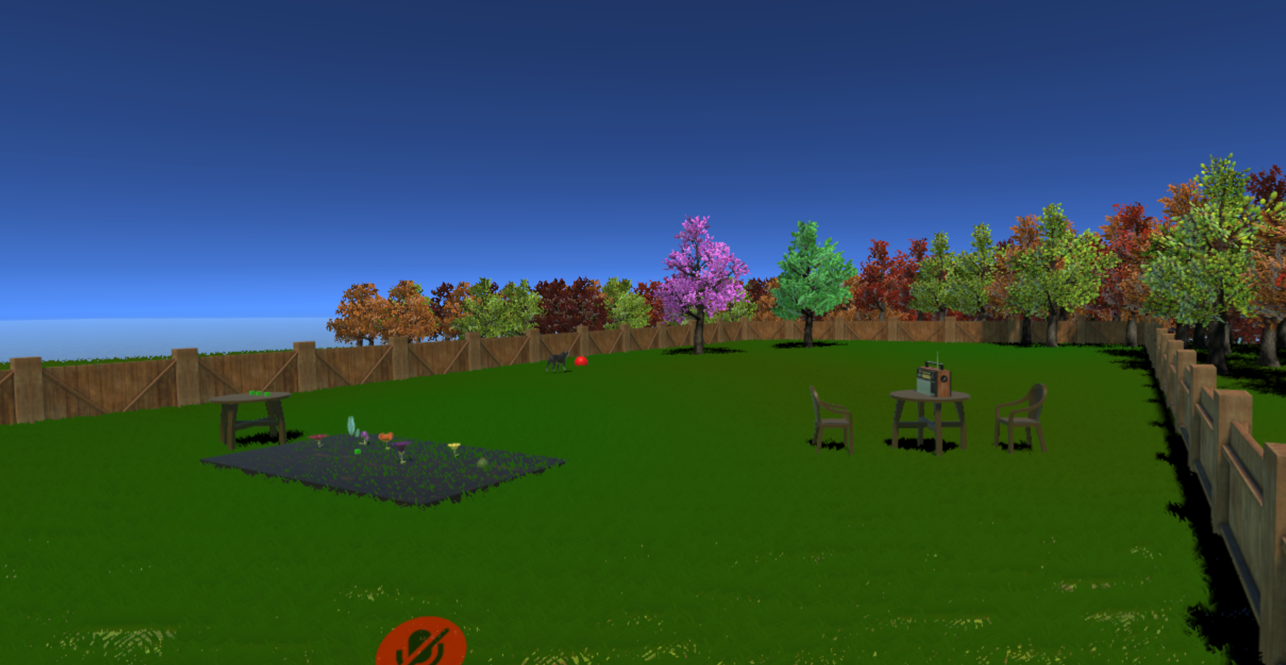
\includegraphics[width=\linewidth]{Images/GardenLife.png}
\caption{Garden Life}
\label{fig:gardenLife}
\end{subfigure}\hfill
\begin{subfigure}[t]{0.3\textwidth}
  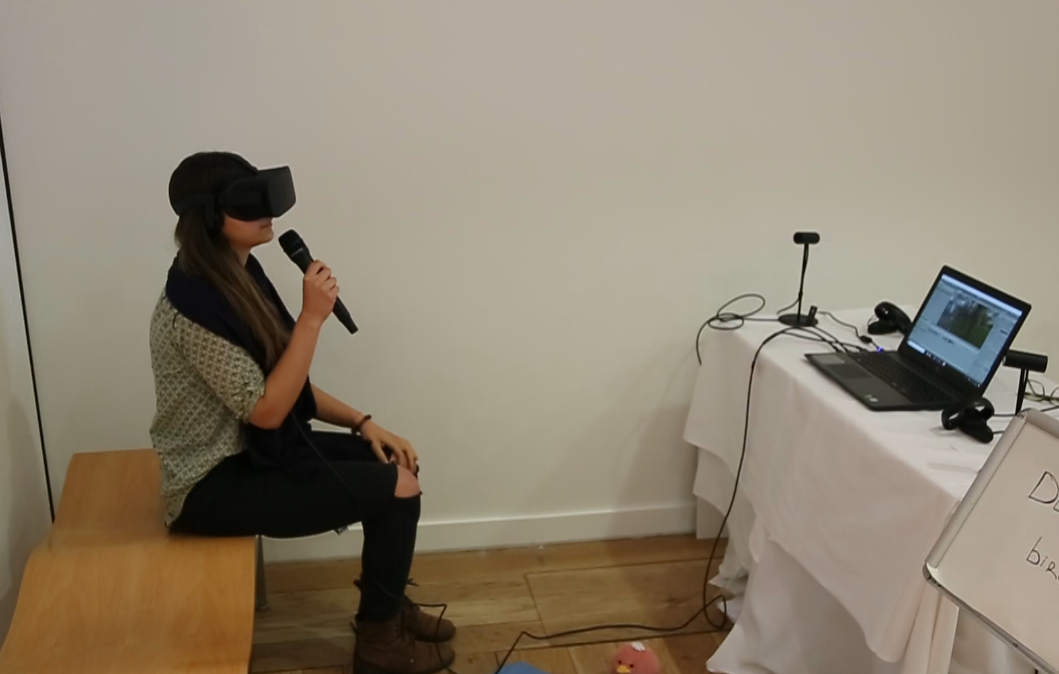
\includegraphics[width=\linewidth]{Images/ChatterBench.png}
\caption{Chatter Bench}
\label{fig:ChatterBench}
\end{subfigure}\hfill
\begin{subfigure}[t]{0.3\textwidth}
    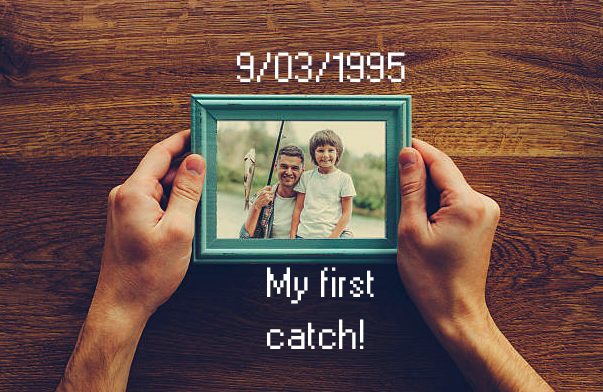
\includegraphics[width=\linewidth]{Images/AugmentedWorld.png}
\caption{Augmented World}
\label{fig:AugmentedWorld}
\end{subfigure}

\begin{subfigure}[t]{0.3\textwidth}
    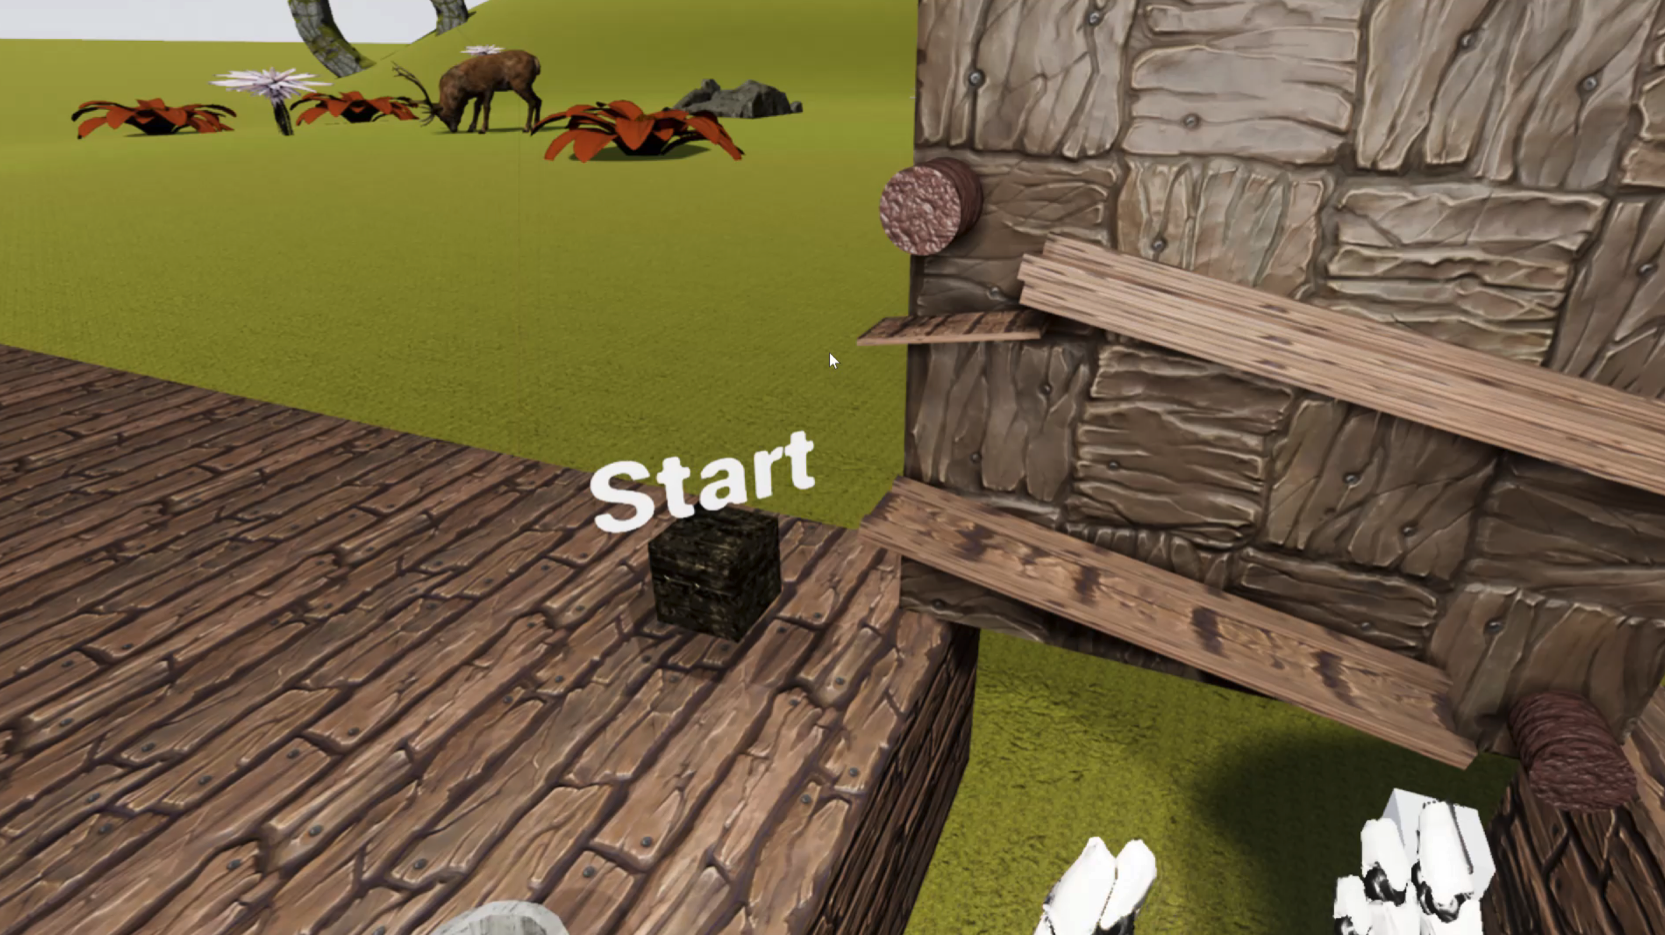
\includegraphics[width=\linewidth]{Images/VRHallucinate.png}
\caption{VRHallucinate}
\label{fig:VRHallucinate}
\end{subfigure}\hfill
\begin{subfigure}[t]{0.3\textwidth}
    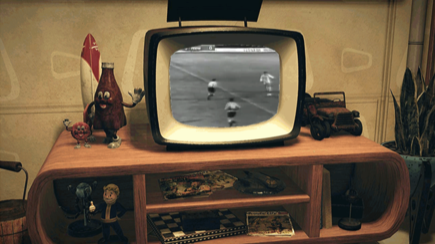
\includegraphics[width=\linewidth]{Images/LookingVRBack.png}
\caption{Looking VR Back}
\label{fig:LookingVRBack}
\end{subfigure}\hfill
\begin{subfigure}[t]{0.3\textwidth}
    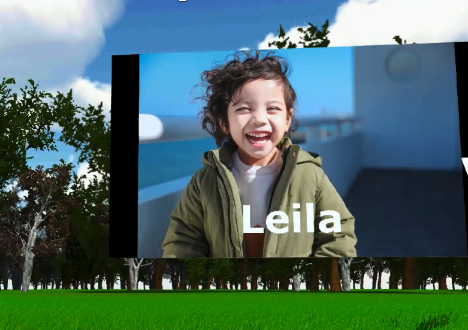
\includegraphics[width=\textwidth]{Images/MindfulForest.png}
\caption{Mindful Forest}
\label{fig:MindfulForest}
\end{subfigure}

\begin{subfigure}[t]{0.3\textwidth}
    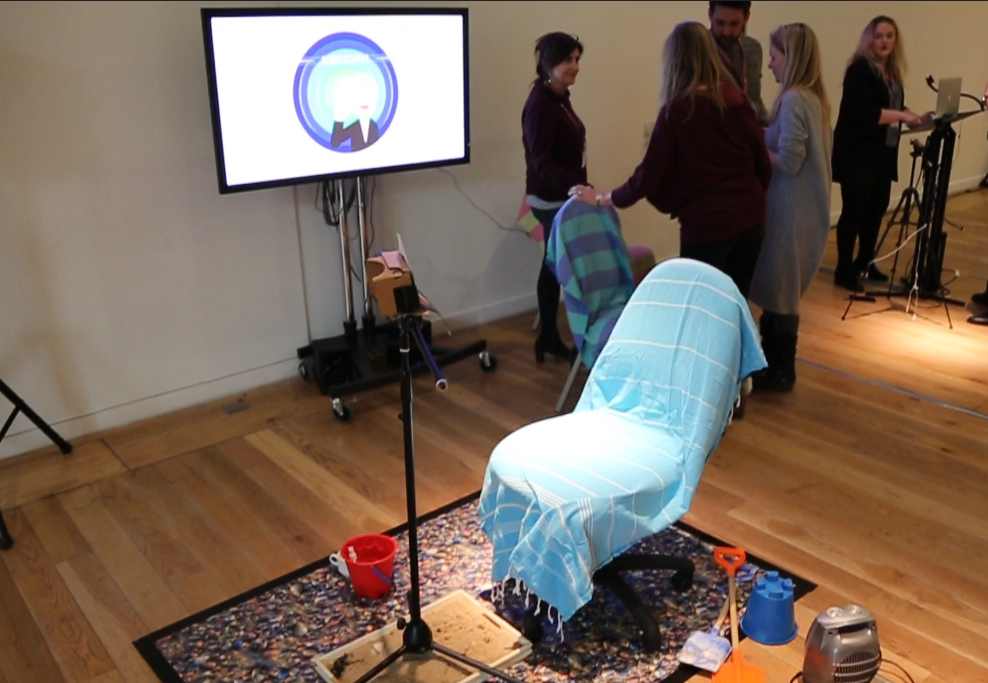
\includegraphics[width=\linewidth]{Images/SensoryTides.png}
\caption{Sensory Tide}
\label{fig:SensoryTide}
\end{subfigure}\hfill
\begin{subfigure}[t]{0.3\textwidth}
    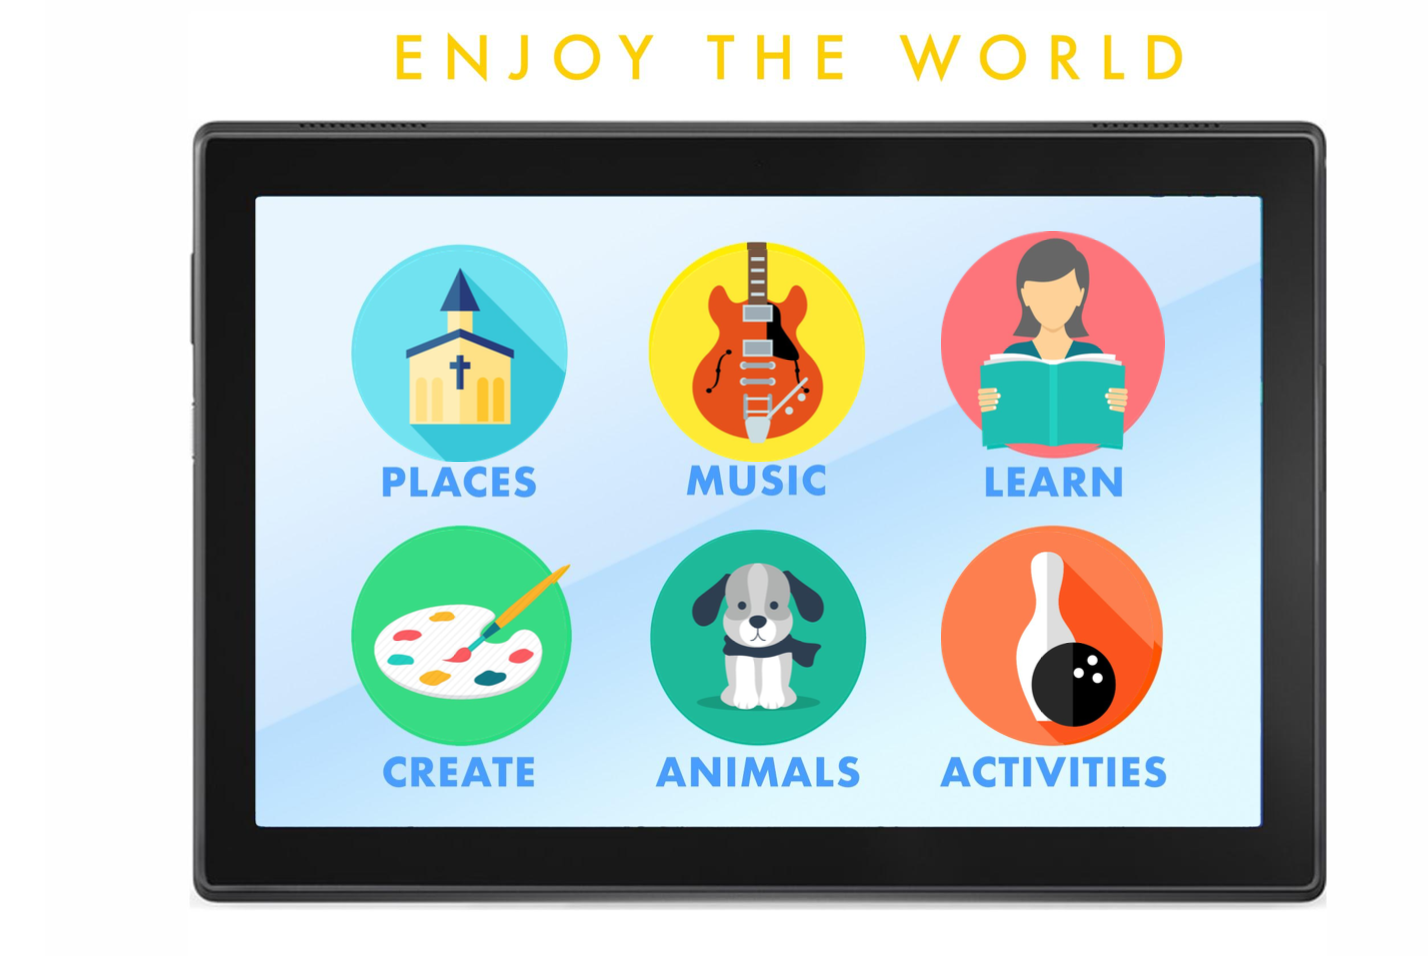
\includegraphics[width=\linewidth]{Images/WorldShare.png}
\caption{WorldShare}
\label{fig:WorldShare}
\end{subfigure}\hfill
\begin{subfigure}[t]{0.3\textwidth}
    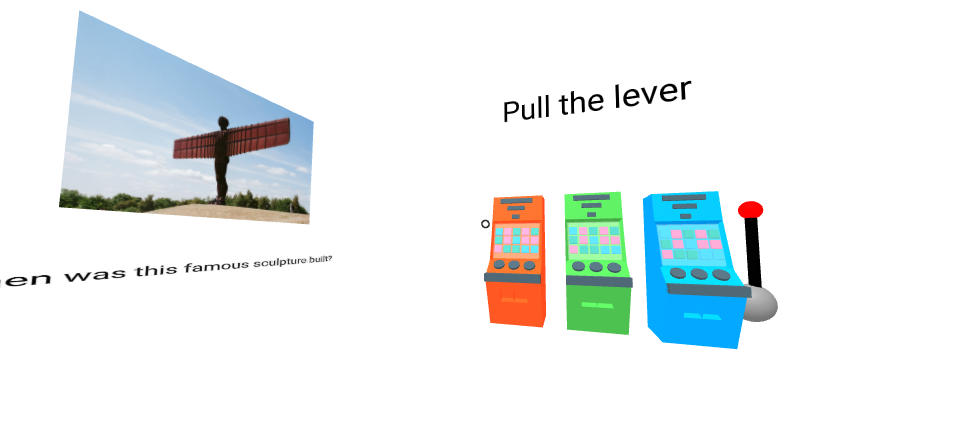
\includegraphics[width=\linewidth]{Images/VRMotion.png}
\caption{VRMotion}
\label{fig:VRMotion}
\end{subfigure}
\caption{DemVR final prototype ideas}
\label{fig:DemVRFinalIdeas}
\end{figure}
From the final nine ideas, each team developed a prototype of their final idea alongside their ten minute presentation. In this subsection, I briefly breakdown each teams' proposed ideas and their final ideas:

\subsubsection{a. Garden Life (seven undergraduate computing students}
\label{sec:gardenLife}
\textbf{Proposed Idea:} Garden Life's proposed idea originated from Ideaboard where their idea would be to \textit{"create a journey through the story of your life using media that links memories with locations."}

\textbf{Final Idea:} In the teams' final idea, they created a VR garden and dog companion for those living in isolation without access to either in real life. The team had considered ways for sharing experiences by carers assisting the growth of a virtual garden through the extension of a tablet while the person living with dementia used VR. Furthermore, the team added multiplayer aspects to the experience allowing family and friends to virtually join the user in their own personalised garden with their virtual dog. 

\subsubsection{b. Chatter Bench (two designer / researchers) - Won 2nd Prize}
\label{sec:chatterbench}
\textbf{Proposed idea:} A chat-based VR experience that will consider the importance of sensitivity and aesthetic design. This idea was not developed on Ideaboard, but came from conversations between the two team members.

\textbf{Final Idea:} In teams' final idea, they developed a shared VR experience in Unity game engine where two users could 'sit' and talk on a virtual bench. Either the care partner, or person living with dementia could select from an array of different 360-degree environments where the two users could talk into a microphone and hear one another.

\subsubsection{c. Augmented World (six undergraduate computing students}
\label{sec:augmentedWorld}
\textbf{Proposed Idea:} A bespoke chronological AR timeline connected to experiences of the users past and family. The proposed idea was developed on Ideaboard by two of the six members who originally focused their idea on themes of reminiscence. 

\textbf{Final Idea:} An AR app that 'enhances' environmental objects to facilitate meaningful social interaction by connecting virtual objects to overlay on the real-life object. For example, a user can scan a picture of their family in the app which will then overlay virtual text or videos onto the picture.

\subsubsection{d. VRHallucinate (six members from developer, researcher, and UX backgrounds}
\label{sec:VRHallucinate}
\textbf{Proposed Idea:} As the team joined the event late and missed the pre-engagement phase, the team decided to develop a gamified experience to visualise hallucination-like effects to raise awareness of potential cognitive deficits that one may get with a diagnosis of dementia.

\textbf{Final Idea:} Similar to their proposed idea, they designed the hallucination game but targeted elements of ways to educate family, friends and the public surrounding the potential challenges of living with dementia.

\subsubsection{e. Looking VR Back (four members from marketing, development, biomedical backgrounds}
\label{sec:VRBack}

\textbf{Proposed Idea:} Using sounds, scents, and colours as a way to support reminiscence - this was proposed on Ideaboard by the same team.

\textbf{Final Idea:} Same idea but used a personalised example relating to Newcastle football game in 1969 as a way to take people living with dementia back to the particular experience through scents, sounds and 60-70's VR room aesthetic. 

\subsubsection{f. Mindful Forest (two undergraduate computing students}
\label{sec:mindfulForest}

\textbf{Proposed Idea:} A fantasy shared experience where families can add videos to trigger past memories. This idea was developed at the event as the team did not engage with Ideaboard.

\textbf{Final Idea:} A forest-like environment with gentle music and scenery. Families and friends can add videos to help with memory stimulation.

\subsubsection{g. Sensory Tide (six members from developer, researcher, and film backgrounds) - Won 1st Prize}
\label{sec:senosryTide}

\textbf{Proposed Idea:} The team combined several participants during the team formation, where multiple Ideaboard ideas came together. At the initial stage of developing their idea, the team had ideas of: replacing VR headsets with full-dome projections, themes of focusing on designing for the moment, as oppose to improving cognitive deficits, and designing reminiscence tools to increase Independence doing tasks.

\textbf{Final Idea:} The team developed an adapted version of a headset to resemble a beach telescope that was easily accessible. Additionally, the team created the VR beach experience to support multi-sensory needs for example, the user could smell seaweed in the room, a heated fan attached to the wall and sand under the feed of the user. 

\subsubsection{h. World Share (three filmmakers}
\label{sec:WorldShare}

\textbf{Proposed Idea:} Developed at the event, the team's initial idea was a tablet-based app to allow people living with dementia to 'travel' across the world and take part in tours and explore other scenic outdoor locations.

\textbf{Final Idea:} The final idea consisting of the following: a tablet that acts as a controller for interaction, and a headset to be used by the person living with dementia. The person with dementia would then request an event or a family recorded experience which the care partner would navigate to on the tablet and send the video/experience to the VR headset.

\subsubsection{i. VRMotion (for members from developer and researcher backgrounds)}
\label{VRMotion}
\textbf{Proposed Idea:} Influenced by their prior work in research, the team's initial idea was care home oriented where the VR experience would be a celebration of abilities of the individual instead of trying to bridge the abilities they have lost. 

\textbf{Final Idea:} Building from their proposed idea, they developed a shared virtual world where people with dementia can take part in group activities such as songs to sing along, guess the place, and solve the riddle - that was inspired by the work of Foley et al. \citep{foley_printer_2019}

\subsection{Reflection}
\label{sec:EventReflection}
Following the event, I began to process and reflect on how the event went and what the contribution was to HCI research. From early on, it was apparent that while the nine teams had created bespoke shared VR experienced prototypes, I felt that the lack of involvement of people living with dementia was significantly reflected in teams' presentations, raising concerns as to how designers/developers may design for dementia without these lived experiences front and centre in their design processes. Given this, it is worth writing that my positionality as a dementia researcher was an integral influence in the hackathon's facilitation and subsequent evaluation of the event \citep{bourke_positionality_2014}. During the study's framing and running of the event, I selected particular researchers who take a similar approach to dementia through using a person-centered design approach. While this was intentional as I wanted to explore ways to scale person-centered approaches, the orientation towards how I view dementia influenced the hackathon's framing by emphasising participants to take a more creative and well-being approach to their design instead of problematising someone's cognitive deficits. Furthermore, I hand-picked the facilitators who also take a more relationship and meaningful interaction to their work instead that of a biomedical one. By carefully selecting particular facilitators and presenters, it is likely that this impacted the teams' final prototypes and potentially limited the potential of teams to develop more biomedical led design approaches. 

In response to the failures and challenges that I faced by attempting to scale/ replicate experience centred design for a hackathon, the following research questions guided my analysis of the event:

\begin{itemize}
    \item \textbf{Research Question One:} How do designers/developers represent people with dementia when solely relying on their own experience or lack thereof?
    \item \textbf{Research Question Two:} What consideration for technology do designers/developers prioritize when designing for people living with dementia?
    \item \textbf{Research Question Three:} What challenges arose when trying to represent the voices of people living with dementia and care partners during the hackathon? What opportunities arose which we may, in time, exploit?
\end{itemize}

\subsection{Data and Analysis}
\label{sec:DataAnalysis}
In the study, I gathered data from three different source: 1) Text data of the Ideaboard ideas (I), including additional comments from participants on the ideas; 2) Keynote, Q\&A and teams’ presentations from the event (P) and; 3) Each team WhatsApp group’s text, images and audio, which were extracted using the built-in Google Drive feature. WhatsApp audio recordings were also transcribed and anonymised by UKTranscription (W). To provide an additional context, I made a set of observational field notes (F) throughout the event highlighting conversations I had with teams and facilitators. The initials (I, P, W, or F) indicate the source of the data in the findings.

\begin{table*}[ht]
\caption{}
\label{table:data collection}
\begin{tabularx}{\textwidth}{@{} Y|YYYYY @{}}
\textbf{Stakeholders} & \textbf{Ideaboard (I)} & \textbf{WhatsApp (W)} & \textbf{Presentations (P)} & \textbf{Field notes (F)} \\ \hline
Hackathon participants & 11 submitted ideas & 25 minutes audio recordings + average 25 texts per team & 117 minutes & N/A \\
People with dementia and care partners & One care partner replied to eight submitted ideas & N/A & 15 minutes Q\&A & N/A \\
Facilitators & N/A & Average 6 texts replying to each team & 40 minutes & 11,355 words \\
\end{tabularx}
\end{table*}
My analytic approach followed a Thematic Analysis (TA) set out by Braun and Clarke \citep{braun_one_2020,braun_using_2006}. Working from multiple data sources, I ordered the individual sets of data across a timeline to make sense of interactions between data sets. This approach helped to decide if it was possible that a certain event, such as a keynote or the Q\&A, had influenced a team's design approach, though our qualitative approach is careful in not claiming causality. Second, the I structured a set of team narratives consisting of the different data sources described above. Structuring the data this way helped to describe the chronological development of each individuals’ teams from design ideation through to presenting their final idea and post-hackathon reflections.  Once the data was framed chronologically, I began to conduct open coding. I then meet bi-weekly with Dr Kellie Morrissey, Dr Sarah Foley, and Dr Dave Kirk to construct themes and reflect on the patterns evident across the data. Finally, the I constructed the named themes, which are presented in the following section. 
\section{Learning from the event}
\label{sec:LearningEvent}
This section presents two overarching themes describing the participants' interactions on learning and designing meaningful shared experiences for people with dementia. The first theme considers participants' approaches to engagement and design: this explores their motivations for taking part in the event, as well as analysing how participants attempted to incorporate their new understandings of dementia into their design. The second theme, reworking participants’ conceptualizations for design, describes the challenges of assimilating these sensitivities into design outcomes, given the absence of crucial stakeholders.
\subsection{Participants' approaches to engagement and design}
\label{LearningEvent:ThemeOne}
As aforementioned in our literature, participation in design events is significantly labour-intensive and time-consuming, yet they remain a popular route for learning and developing new paths to research. For the majority, participants had very little experience of dementia which required the support of learning on topics of dementia and VR. While this may suggest a steep learning curve for engagement in the event, participants continued to work throughout the event to build their working demos and presentations. To this point, the following subthemes describe what motivated participants to spend their weekend ‘hacking’ away and how learning about dementia impacted their design approaches throughout the weekend.
\subsubsection{Motivations behind participation}
\label{ThemeOne:subthemeOne}
Participants’ motivations for taking part in the event ranged from their own personal experiences of loved ones with dementia, seeking a chance to win the cash prize, sharing their voice, and learning about the area of dementia \& HCI. For those with personal experiences, their motivation was typically driven by family members having dementia or having worked in the area of dementia. For example, in team World Share presentation, they described conversations with their Grandmother about his Grandfather where \textit{“he may not remember going to the beach that day but he’s happy, and it’s about the day-to-day quality of life, which is something we’re looking to do with [our idea]” (P)}. Likewise, team Chatter Bench described family connections influencing their involvement where they \textit{“called [his] mum [to talk about his] grandparents who were living with dementia in a home before they died…this informed what was important [to them joining the event]” (P)}. For others who had experience in the field from a research perspective, their reasoning for taking part was rooted in learning how VR could be a beneficial technology within this space. For instance, one member from VRMotion works on \textit{“intergenerational interactions in dementia care” (P)} and came to the event to \textit{“learn how VR and dementia can be linked together” (W)}. Undergraduate teams echoed similar comments where VRHallucinate could learn about \textit{“how technology can help dementia” (W)}, or GardenLife asking, \textit{“What can I do to help people with dementia?” (F)}. 

At the end of the event, GardenLife expressed their hopes that \textit{“events such as this and research continuing to deepen our understanding of these issues will help to alleviate the stigma that caused [negative representations] to happen" (W)} presents a series of motivations that participants are keen to learn and educate themselves on sensitive issues. Perhaps unsurprisingly, a sense of competition and prize money were significant motivators for several teams. The first author’s field notes described \textit{“how they [teams] would come up to [first researcher] and say they’re going to win the prize money as their idea is the best” (F)}. While this made for particularly enthusiastic participants, in many ways, it could also be seen to hinder collaboration between teams. Moreover, it was also a potential contributor to why there was little uptake from our participants for using the online platform, which would have made participants’ budding ideas public knowledge. During our team formation, the first author was getting to know one of the six members who later made-up team Sensory Tide, when they had mentioned how three of the team members had \textit{“got together and had a few meetings, but [their] idea is top secret. [they’re] not gonna share it till we have to” (F)}. Teams’ secrecy in their ideas constrained their willingness to share their ideas publicly before the two-day hackathon in fear others would copy or otherwise be influenced. Similarly, the team that dropped out during team formation had similar concerns of revealing their idea to the extent of questioning \textit{“who owns the intellectual property” (F)} of the idea. 

To provide engagement for people with dementia and care partners, we set up our ‘pre-engagement phase’ that included an online platform, and in-person workshops. As we described in our recruitment, only one of the twelve participants who signed-up to our online platform (Ideaboard) was not a designer/developer. Our one care partner – Denis, was motivated to share his experiences of his father’s dementia hoping outputs of the event would provide \textit{“published prototypes [he] can use [with his father]” (I)}. As Denis continued to comment on the Ideaboard ideas, he would express limitations in people’s ideas saying:\textit{ “my father is too old to use social media” (I)}, or \textit{“my father wouldn’t understand how to navigate in VR” (I)}. In these examples, Denis was advocating on his father’s behalf to make sure his father’s differences may be considered in future VR outputs. Although Denis felt comfortable to share his experiences, several participants without experience of dementia sent emails asking for advice on their ideas before they submitted as they were worried, they would be \textit{“embarrassing [them]self” }from their lack of knowledge around dementia. Although they expressed, they’d \textit{“really love to be involved and help to make a difference”}, the sensitive nature of the topic at hand made some participants question their ideas and hope that they \textit{“hadn’t got the wrong end of the stick”}. Similarly, the first author’s field notes indicate that “\textit{participants seemed anxious or uncertain if they’d be saying the right thing [online] which might be why they didn’t engage” (F)}. Although several teams felt uncertain to share their ideas or take part in the online platform, participants were still motivated to take the time and conduct research before the event, whether that was GardenLife \textit{“reading VR and dementia papers” (W)}, or how Augmented World had sought guidance from a Dementia Advice Centre about VR as a potential viable technology for people with dementia. Additionally, our planned in-person workshops co-organized with a local dementia café raised concerns for participation when \textit{“no-one signed up to our workshops... CEO of the café just notified me and asked if we should cancel the [the workshops]” (F)}. From the first authors field notes, at the time, they felt \textit{“perhaps members [of the café] are no longer interested in VR work anymore”}. However, even if so, the research team received nine emails after the event from companies/individuals asking if any ideas had gone into \textit{“production”} or any of \textit{“the outputs from the event are in digital form”}. Many of these companies specialized in providing \textit{“care across a number of homes”} but reached out looking for cheaper solutions. Participation was scarce in the pre-engagement phase which initially presented that\textit{ “perhaps people are no longer interested in VR?” (F)}, and while this may have been the case for our workshops (that we discuss in our discussion), Denis’ motivation and companies interested in what the event had created suggests maybe the lack of support to learn dementia prior event hindered participants motivation to engage online. This theme describes the motivating factors influencing participants to take part in the hackathon. While there are examples of personal and educational motivations behind taking part, this themes also raises concerns about the type of incentives expected in a typical hackathon event. For example, though prize money motivates taking apart, it hinders the sharing of resources and knowledge between teams as this may affect the competition outcome. However, although our event may not have gained as many participants as it did without prize money, there are some instances of teams’ going out of their way to initiate conversations with care partners or sharing their personal experiences in the hope to have a say on the hackathon’s VR outputs, indicating that at least some of our participants’ motivations were pro-social in nature.
\subsubsection{Participant implementation of these new understandings}
\label{ThemeOne:subthemeTwo}
In our pre-hackathon stage, the submitted ideas formed an initial picture of how prospective participants viewed dementia – for instance, through their idea helping to \textit{"making them [people with dementia] feel more independent"}, or to \textit{"help calm the mind[s]"} of people with dementia \textit{(I)}. Although multiple participants used terminology no longer accepted in best practice in dementia, such as \textit{"sufferers"}, and\textit{ "patients" (I)}, the design ideas uploaded suggest these terms are not intended to stigmatize. For example, a participant from team World Share suggested ways for VR to \textit{"guide sufferers through daily basics" (I)} in order to reduce the effects of memory loss by having VR technology allow them to repeat tasks such as \textit{"basic cooking, making a cup of tea" (I)}. Although these terms were being used early in the two-day hackathon as well, through engaging in conversations with facilitators, and through introducing resources such as the DEEP Guide \citep{diaries_deep_2020},  participants changed their language and used more respectful, person-centered terms. In the same vein, many early iterations of participants’ ideas promoted 'treatment', 'fixing the disease' and ways for technology to improve a person's memory or other deficits \citep{hendriks_valuing_2018}. Throughout the event, several teams, particularly those made up of undergraduates, expressed their interest in learning from academic papers. For example, Mindful Forest described \textit{“a research paper about this care home in Sweden, that took outpatients in the forest and found patients communicated more and remembered more about it” (P)}. This paper inspired them to create a forest environment for their final design. While facilitators assisted in suggesting particular papers or articles, it led to GardenLife initially designing for ways to link memories to locations, to develop and ideate on social complexities of feeling \textit{“silly” or “scared” of using VR – and to find a solution of “easing [the user] into the experience” (P)}. Through initial facilitation, conversations, presentations and inspiration packs, World Share described their interest in understanding the\textit{ “the challenges, accessibility, interactivity, and limitations around dementia care the people around people with dementia” (W)}.

Additionally, teams’ design decisions were influenced by conversations with stakeholders before and during our hackathon, such as Howard’s Q\&A, discussions on Ideaboard, or reaching out to caregivers outside the event’s network of people. For example, Augmented World designed for AR rather than VR based on advice from a Dementia Advice Centre, which suggested: \textit{“VR might be quite frightening…and with it being a bigger adjustment mentally with them living in a reality they don’t know what is real or not” (P)}. Similarly, Michael – a team member from Sensory Tide - engaged with Denis via Ideaboard to gain a richer understanding of dementia from a care partner’s perspective. Denis highlighted ethical and financial concerns for Michael’s proposed idea on Ideaboard: this was to create\textit{ “full-dome projections” (I)} as an alternative to \textit{“wear[ing] VR headsets” (I)}. The care partner and the designer engaged in conversation on the platform and raised concerns about projection domes’ practicality for care homes. The care partner pointed they are \textit{“\$13,000 as base price” (I)}. The team shifted their course from here, and their final idea was by developing light-weight DIY solutions through the use of Google Cardboard. During Howard’s Q\&A, VRHallucinate started to link prior knowledge of hallucination research and aligned it with Howard’s shared experience of hallucinations he has been having recently. While the team initially identified similarities between their understanding and Howard’s stories, when he opened up about how his friends\textit{ “disappeared, and only three people still keep in touch” (P)}, the team altered their idea, shaping it instead about being how VR could \textit{“teach [people with dementia and their care partners] to experience these visual uncertainties and inconsistencies, by playing a problem-solving game that will manipulate and change as you play to signify a change in hallucinations” (W)}. 

While participants demonstrated new understandings of dementia and how they may design for this care context, adopting this critical approach in their design proved challenging for the teams. In fact, the only teams who demonstrated this critical sensibility are the ones populated by experienced dementia researchers. The two winners of the hackathon - ChatterBench, Sensory Tides and team VRmotion could pull from their successes and failures in the area and critique their ongoing design decisions. For example, Sensory Tides took inspiration from the many language guides around dementia and considered what that would mean for the term ‘Virtual Reality” (see table 3 for final idea). Aware of the social complexities that people with dementia may face with defining their reality and the concerns that earlier academic work had with the terminology surrounding Virtual Reality, the team designed for continued reassurance through the technology instead. Instead of the term VR, they describe their experience as a “magical viewfinder” (P) along with giving calm and helpful suggestions of how users may use it: either by leading the experience through the viewfinder or “lean[ing] back away from the headset and join everyone else relaxing on the [virtual] beach” (P). Similarly, Chatter Bench and VRmotion began to question some of the more ethical and social challenges of designing within this space. The teams questioned, “How are you going to fit [the experience] into the [care home’s] schedule?” (P), or VRmotion considering “who controls [the experience], why would the person with dementia control it?...How would a facilitator involve themselves into the experience?” (P). In the teams’ final presentations, Chatter Bench raised concerns that their idea may add “strain on the family and resources” (P) in order to create the 360-degree worlds that people with dementia and care partners may want to share together – to the point that Chatter Bench presented future ideas of more social and community-led curation methods to generate a variety of environments in the “hope it will scale” (P). Although the event provided participants with curated research papers, ‘snippets’ of the lived experiences of people with dementia, and resources such as the DEEP Guide, these reflections can only offer examples of best practice rather than develop genuine understanding and relationships that may mirror the type of experiences the researchers suggested they had.  The extent to which we can support participants to both learn about a complex issue and apply this new knowledge to design within the traditional hackathon structure warrants further consideration. We return to this reflection in the discussion. 
\subsection{Reworking participants' conceptualisations for design}
\label{LearningEvent:ThemeTwo}
Through our event, we had hoped to engage with people with dementia and care partners in order for developers/designers to have the opportunity to gain insight into what priorities or interests they should keep in mind when designing their shared VR experiences. However, as we have described in our paper, we did not manage to involve care partners and people with dementia in the ways that we had hoped. As a response, the following subthemes describe the subsequent consequences of a lack of engagement with lived experience, where teams had to adopt different approaches to design for an absent user. Furthermore, we discuss the outcomes of designing for users who are not present, highlighting how designers returned to established ideas of deficit models of dementia. 
\subsubsection{Constructing the absent user}
\label{ThemeTwo:subthemeOne}
Teams’ ideas shifted over the course of the event as their interactions with facilitators, inspiration packs, and Howard unfolded; we noted that participants often focused on particular comments made by speakers who discussed their experiences with people with dementia. The interplay between the stories, resources and conversations scaffolding the event helped to create an initial understanding of what it might be like to live with, and design for, dementia. However, by having a lack of people with dementia and care partners at the event or through engagement on the online platform, a number of teams pictured the person they are designing for on Howard’s experiences of dementia that he shared in his 15-minute Q\&A. For those teams, Howard became a pivotal resource, and a somewhat static personality they were designing ‘for’. The ways in which teams reacted to Howard’s experiences varied. Team Garden Life changed their design approach in response to Howard's hobbies and interests: their initial idea centered around "a journey through the story of your life using different media that links memories with locations'.” They stated that “The experience can be customized by family, so that the focus is on either neurological rehabilitation or reminiscence" (I). 

In response to Howard’s Q\&A, the team developed a virtual reality ‘garden’, with a feature that allowed the user to interact with a virtual dog. In the WhatsApp group chat, the team state that they "found it interesting [Howard] has a pet dog" (W). This led to the team reflecting on how people living in a care home may not get that opportunity, but that "having an animal to care for seems to help people in a lot of ways' (W)'; and the team felt a virtual dog could help with loneliness. As the team developed the garden environment further, they built customizability options: “you can change its breed, colour and name of the animal" (W). Similarly, while Mindful Forest didn’t focus entirely on Howard’s experience, Howard’s experiences provided an opportunity to expand their current understandings of dementia as they “realized [they] actually don’t know as much [about dementia]” (W). In response, the team’s final idea featured “family members adding various pictures from holidays when they were young, so it would help in remembering if they forgot about their grandson or grand-daughter” (P). While the team prioritized their experiences of dementia where “I still remember the day when my Grandma no longer recognized me” (P),  the team were inspired to enhance their social features after being “surprised that all of Howard’s friends left”.  While basing design decisions on personal stories, or on Howard’s is not necessarily harmful, the lack of interaction with a variety of people with dementia limited the space for creativity and exploration, and instead presented Howard’s or participants personal experiences as a ‘one size fits all’ persona for dementia. Further, our event overlooked involvement of care partners, health care providers and friends who may be involved in the ecology of care which limited teams such as Chatter Bench describing they ‘have no understanding of how a nursing home really works”. 

For the most part, teams' initial ideas as outlined in the methodology are centered around cognitive training and reminiscence, except for three teams – VRMotion, Sensory Tide and Chatter Bench. Perhaps coincidentally, these three teams had at least one researcher with a background in working with people with dementia who could not only draw on their prior experiences, but also had extra insight into current research in HCI and dementia care. The three team’s shared design focus of \textit{"being in the moment"}, or \textit{"celebrating what abilities are left"} are not particularly novel contributions to dementia research, but they speak to the participant’s knowledge of the best practice in care. With that said, even though Sensory Tide and Chatter Bench won the final prizes, they still struggled to construct an understanding of who the user might be. During their final presentation, Sensory Tide presented a set of personas that often abstracted the user and were prone to stereotypes such as: \textit{“Mary: can often get confused or lost if left alone” (P)} and \textit{“Ben: has anxiety and depression as a result of his diagnosis (P)}. Although personas can be useful for designers to connect with the people they are designing for, it shows that even the winning teams were limited to representing the person with dementia as a set of stereotypes based on their diagnosis. Although Sensory Tide used the personas to \textit{“help us decide who we are actually designing for”}, for reasons similar to Chatter Bench, they found it \textit{“hard to figure out what to design because [they] can’t ask the user” (W)}. This observation goes a way towards highlighting the value teams placed on engaging with end-users in the research, and highlights what is at the centre of this finding: the perceived importance of engagement between designers and stakeholders. In our final sub-theme, we describe the continued effect that the lack of stakeholder involvement had to designer’s creativity as they prioritized risk aversion as opposed to exploring a range of possibilities that people with dementia may want to experience. 
\subsubsection{The trade-off between autonomy and safety}
\label{ThemeTwo:subthemeTwo}
Some teams raised concerns regarding how best to represent an appropriate environment virtually for users with dementia. This often resulted in taking an inherently ‘safe’ design approach in order to reduce any 'negative' or 'confusing' experiences, thereby ensuring neutral or positive emotions. For example, team Chatter Bench were conflicted in \textit{"how [to] represent the person living with dementia [in VR]" (W)}. The team's idea is a ‘VR skype call' where both participants would be present in a 360-degree video on a bench in a park. Members of this team were attuned to the technical aspects of design, having worked in VR over the past five years, where the concern of the illusion of embodiment and the representation of the user's body has been regularly discussed \citep{nakamura_virtual_2019}. For example, when discussing the possibilities of designing avatars for the VR environment, they worried that, \textit{"the other [avatars in the environment] will look like a scary apparition or, you know some floating smiley head" (W)}. To tackle this concern, the team removed the virtual avatars and transmitted only the online voices between the two users. The team suggests their decision was to some extent a trade-off: when you are already \textit{"placing a headset on somebody with dementia”} (and therefore causing some discomfort in all likelihood), \textit{“you don't want to take it to a further extreme when you're showing, magic hands popping around or magic heads" (W)}. Despite ‘magic hands’ and ‘floating heads’ being common way to represent the user in VR, the team remained skeptical of this approach due to the common conception of people with dementia as unable to decipher what is ‘real’, and what is not, in both real life and in VR. Similarly, team Mindful Forest, state that they originally \textit{"planned to add fantasy elements to our idea. But due to learning about other symptoms like hallucinations, we, therefore, had to change it to be more realistic, because we don't want to cause any problems for people with dementia" (W).} Both teams were focused on the person’s safety, deciding that this was more important than designing for autonomy or ideas of abstract aesthetic engagement. In both instances, designers took the decision-making process out of the user’s hands by removing fantasy elements or bodily representation in VR to prevent harm. While user’s safety is a priority in any form of design process, removing the option of switching features off or on can be argued to restrict the expression of individual differences and limits the potential autonomy a person with dementia may have over the experience.

Many teams whose ideas sought to involve care partners, families or friends would often make design decisions that shifted the responsibilities of setting up the technology to the caring role. Again, while this may be useful or even preferential for some, it may also result in a loss of agency for the person with dementia. For instance, team Chatter Bench stated that if their VR experience was implemented into a care home, then scheduling of the VR 'Skype calls' need to consider \textit{"fitting into the schedule of the care partner as well" (W)}. The team realized that a diagnosis of dementia often brings along with it a shifting of responsibilities, with these being placed instead upon others such as their care partner, potentially further eroding the autonomy of the person with dementia and contributing to caregiver burden. Alternatively, team World Share focused on their interactive app consisting of events, family and friends’ recordings to be as customisable as possible to \textit{"approach the widest possible audience" (P)}. World Share's approach wanted the user to have as much ownership and agency when using their VR system as they argued \textit{"just because you have dementia, does not mean you don't want to learn. You want to be able to explore these things" (P)}. Although this idea encourages customisability to tailor the system to the user, it could also be argued that placing all the decision-making processes on the individual may also hinder or overwhelm the user through exploring the system. In sum, the majority of teams found it challenging to design VR as a shared experience particularly when trying to place responsibility on who drives the experience – the person with dementia, or the care partner. 

However, while they still found it challenging to navigate the space of shared VR experiences, Sensory Tide designed their VR experience with reference to experiences both of families living with, and those with dementia. In this instance, as the person with dementia controls the movement of the VR headset, this drives the experience for not only themselves, but projects what they are seeing into the outside space of the room for the family to see.  Similarly, VRMotion designed a series of VR activities such as “songs to sing along to, guess the place, solve the riddle or even share jokes”, and considered the collaborative decision-making needed to ensure continued participation within the care home. This is done through giving the staff member the responsibility as a facilitator to “pull a lever on a [VR] slot machine, which will show a random task. [Then] people with dementia and the facilitator will work together to complete the task”. These examples highlight difficulties that may occur when designing for decision-making, where the two extremes are to either place all the responsibility onto the care partner through risk-averse approaches or giving full responsibility to the person with dementia to aid their autonomy. However, in some cases, such as VRMotion, they considered ways to maintain reciprocal interdependent relationships where the person with dementia is part of the decision-making process resulting in a more collaborative experience through not only the experience, but the set-up and responsibility of actions. Our analysis presents the nature of participation from team members, and the impact of structural factors of the event on design outcomes. We explore the different reasons participants were motivated to participate in the hackathon. Motivation for involvement ranged from personal experiences to learning, albeit collaboration between teams being hindered by competition. We also compare participants’ ways of incorporating their new understanding of dementia into their design ideas in order to highlight critical differences between those with and without extensive experiences of dementia. Finally, as an outcome of the lack of engagement of people with dementia and care partners in our event, our second theme describes how teams attempted to design for the absent user through different means, showing that teams fluctuated between values of safety and autonomy when designing for people with dementia. Overall, these findings raise some important considerations for design events such as best understanding participant involvement, designing for the ‘absent user’, and redefining what collaboration may be between different communities, which we further discuss in the next section. 
\section{Considerations for future events}
\label{sec:ConsdierationsEvent}
The findings highlight the fluctuations in participants' conceptualisations of people living with dementia and their care partners: from seeing dementia as a medical issue, to highlighting the more societal issues that arise through stigma. In any case, teams' presented a challenge to comprehend and mold their final user in order to fit them into achieving the hackathon's challenge - to \textit{"to design shared VR experiences for people with dementia and their care partners}. In doing so, several teams either held onto Howard's Q\&A as he was the only present person with dementia at the event, or developing a 'persona' by entangling their experiences with dementia and to those of the facilitators at the event. In multiple instances, the process to deal with the 'absent user' resulted in static persona's that responded to the problem the VR experience would solve. In this section, I will describe a series of research considerations that may respond to the challenges and failures I encountered through the hackathon. Within these considerations, I raise conversations on ways to design \textit{with} as oppose to design to \textit{be like}, alternative approaches to meeting participants where they are, and finally considerations for future collaborative design events. 

\subsection{Designing `to be with', not `be like'}
\label{sec:considerationbeWith}
From early into the hackathon, teams approached their ideation in a varied set of ways in an attempt to best guide the ways in which they structured the person with dementia and their care partners. For instance, Sensory Tides designed a series of personas to illustrate who their VR experience was targetted towards, while GardenLife curated their user based on Howard during their limited 15 minute Q\&A. Maarsden \& Hagg (2016), describe the use of personas and other tools alike, have \textit{"contribute[d] value by informing design, i.e. ha[d] a predominatly prescriptive function... they are meant to open design spaces by connecting the designers with the people they are designing for'}. \citep{marsden_stereotypes_2016}. However, while personas are beneficial in imagining the people you may be designing for, they are prone to stereotypes that is further emphasised to elucidate technological solutions to the challenges at hand. Further x describes that \textit{"once a stereotype has been activated it can shape the predication's we make about people and situations".} As described in the findings, even the teams' with significant dementia research knowledge were prone to stereotypes for example while this is a well defined persona by team \textit{Sensory Tide}, it lends itself to appeal to 'priming' certain problem areas that the team want to tackle in their VR shared experience.
\begin{quote}
\textit{Mary is 81 and lives in Forest Hall with her husband Joe. She has two sons who live close by and visit her almost daily; her granddaughter Rachel also visits regularly with her 7-year-old daughter. Mary has been living with Alzheimer’s Disease for around 5 years now. She enjoys being social and being included in conversations, but it is sometimes clear that she doesn’t always follow what is being said. She will often forget people’s names and where she had put things, and can often get confused or lost if left alone. For the last few years her husband has been doing most of the household chores and caring for Mary, but he has recently had some health problems which means he is a lot less mobile. Both Mary and Joe enjoy being around people and being outdoors, but they now need to rely on other people to bring them places following Joe’s illness. Neither of them are particularly technology literate. Joe has a basic mobile phone for emergencies, but they do not own a computer. }
\end{quote}

While their persona paints a well defined person with dementia and it is apparent they are pulling from their vast knowledge of the area, making their personas \textit{"neither technology literate"} or the husband to be \textit{"doing most of the household chores and caring for Mary"} creates clear problem statements for the experience to fix such as their VR experience being assisted by the person with dementia's care partner, or an attempt to make VR technology as easy as possible to engage with. While they are important prompts to consider, it overlooks the possibilities of more enriching design responses such as teaching people with dementia and their care partners about technology to provide Independence towards not relying on others. 

Additionally, I provided teams' with a  series of resources in hope to provide the designers and developers with creative approaches and learn more about dementia. Mentioned in the methodology, the resources consisted of guides on how to talk about dementia \citep{diaries_deep_2020}, method approaches pulled from IDEO Human-Centred Design toolkit \citep{ideo_2021} such as 'framing your design challenge', 'storyboarding', 'role playing'. The design toolkit  echoes similarities of other toolkits such as IDEO's 2018 work on car play that set out  to \textit{break down the bias} surrounding disability through the development of deck of cards called 'Adapt-o-pack'. In this card game, users select from six different persona cards of a person with disability and pair these with workplace settings such as farming that are intended to challenge the narrative of what people with disabilities can and can't do. Developed in parallel with the authors PhD, they state:
\begin{quote}
\textit{
It is impossible for a person without a disability to ever truly understand what it means to be disabled. Period. True empathy, however, can often take the form of human connection over a shared emotion or experience. The Adapt-o-Pack creates this moment of connection by tapping into the creative potential of the participant, and encouraging them to, even for a moment, empathize with the type of creative necessity people with disabilities display on a daily basis.
}
\end{quote}

While the author argues the limitations of toolkits for providing 'true empathy' or that it cannot replace the experiences we may have with the people we are designing for, toolkits present an opportunity to offer opportunities of creativity and sympathise towards the users they are designing for. In a similar way, our use of a Q\&A with Howard provided participants an opportunity to sympathise and reflect on the challenges that someone with dementia may face. In our findings, I described how for many, this was a turning point for them in realising that they want to help on topics of stigma, loneliness, and opportunities to socialise with other family members. 

However, even through involvement of more evocative design methods, and providing opportunity to listen to Q\&A with a dementia advocate, teams' still developed 'static' personas that ended up being inspired by Howard's life and experiences. For instance, \textit{Garden Life "found it interesting that [Howard] has a pet dog"}, and proceeded to develop an VR experience with a 'companion VR dog' feature  where the user could "\textit{change its breed, colour, and name"}. This is an almost exact translation of Howard describing how his new pet  dog has been providing him with something to do and joy, and while the team did acknowledge that \textit{"having an animal to care for seems to help people in a lot of ways"}, they are unable to delve further  due to  the absence of other people with dementia present, lack of personal experience and overall a lack  of time. The adoption of  human-animal relationships into technology has been a common approach in care and dementia - particularly, it is contrasted with Lazer et al. \citep{lazar_rethinking_2016} work on robotic pets for older people. In this study, older people expressed robotic animals would  happily fit into places they had a momentary need for that included \textit{"cuddling and petting"} to offer opportunities to facilitate new social encounters. However, participants rejected the idea of robotic companions replacing humans or pets particularly when it comes to a solution to loneliness. This isn't to say that Garden Life did a poor job, or that VR experiences cannot at all provide these sort of qualities; but that the team were  disadvantages by the time and lack of engagement with a variety of people with dementia - resulting in overlooking important considerations of how may the technology fit into someones life. Rather than being a substitute for a pet, how could such activities overlap and eclipse with real-world interactions with other peoples pets in order to maintain the multiple psychological and physiological benefits that outside and social engagement brings \citep{gilliard_transforming_2011}.

Beyond this, my findings describe how some participants' solutions led to being risk averse. For instance, \textit{Chatter Bench} were worried about the \textit{"strangeness"} of bodily representation in VR and \textit{Mindful Forest} went against their initial fantasy elements for fear of triggering hallucinations. While the safety and comfort of our participants should be paramount in our minds as we  design new technological responses, a heightened focus on risk might quash  creativity, remove any room for individual differences in user experience, and further limit the expressive and aesthetic potential of the technology itself. It has been noted in prior work, that the presence of risk limits participants' creativity when critiquing, problem finding, and see new patterns. However, not only does this effect design, it may also lead to a cycle of stereotypes in design features and in interactions instead of seeing dementia as a condition of possibility. 





- instead of seeing dementia as a condition of possibiltiy

With Hartman, we see that the design accounts of empathy work create their own scenes of dissipation. They help elucidate how designers may have a particular interest in accessibility and disability, but only partial understanding of their interlocutors’ identities. In retelling the story with disability brought close for inspection, designers may frame disability as the defining characteristic. From this perspective, people with disabilities serve as spectacles for designers to look upon for inspiration. They become important for evidencing that empathy was done and that its benefits could be reaped.


It will hopefully convey the helplessness of those diagnosed with dementia, as there is no cure – the end is inevitable. However, I’m also hoping I can convey that, although we’ve been diagnosed, people like me still have a substantial contribution to make; we still have a sense of humour; we still have feelings. I’m hoping to show the reality of trying to cope on a day-to-day basis with the ever-changing environment that dementia throws at those diagnosed with the condition. Living as well as you can with dementia is all about adapting. Adapting to new ways to enable us to live better for longer with dementia.




\begin{enumerate}
\item \textbf{Disseminate our research in less 'static' ways to offer participants new explorations into ethical and embodied topics of dementia}. To get the public to engage with the more sensitive and complex topics, taking an alternate approach to presenting our work such as through theatre, zines, and other creative arts methods may result in a set of work that provokes similar understandings that researchers aim to gain from working alongside people living with dementia.
\end{enumerate}

\subsection{Unplatforming}
Hello, how are you doing today? Im doing good thank'm

\begin{enumerate}[resume]
    \item \textbf{Meeting your participants where they are.} Instead of designing additional online platforms, consider asking your participants what platforms they would like to use for engagement. Not only does this reduce development costs, but this also provides the opportunity to understand the communication processes your participants are familiar with.
\end{enumerate}

\begin{enumerate}[resume]
    \item \textbf{Involving participants in the entirety of the research process to set agendas and priorities.} Inviting and involving participants in the research process will help to ensure agendas are more closely aligned with the participants priorities and desires. Further, participant-led research may offer understandings into new, more impactful ways our research be of benefit to communities beyond academic publications. 
\end{enumerate}

\section{Conclusion}
\label{sec:Conclusion}